% Почему нам недостаточно познакомиться лишь с современными представлениями о методологии исследовательской деятельности и ее социальной организации? 
% Это нужно, чтобы понимать, чем мы занимаемся, когда занимаемся наукой. 

% Сможем ли мы
% по-настоящему заниматься наукой, если для нас она будет чем-то не вполне
% знакомым?
% Как можно спросить, сможем ли мы по-настоящему понимать человека, если
% толком не знакомы с ним? Мы вроде работаем бок о бок каждый день, знаем его имя,
% как он выглядит и так далее, но совершенно не представляем, как с ним быть, чего
% от него ожидать, как выстраивать коммуникацию. Точно так же, как про интересного
% нам человека, мы хотим знать что-то о его прошлом, причем не просто факты, там-
% то тогда-то родился, он столько-то пошел в школу, ходил в какую-то секцию, то мы
% хотим узнать о его переживаниях, о его детских воспоминаниях, о его друзьях, его
% страхах, кризисах, их преодолении, словом о том, как он формировался, на
% основании чего принимал судьбоносные решения и каким образом поступал в сложных
% ситуациях. Тогда и информация о датах, цифрах, именах не так важна для понимания
% человека. А, собственно, что важно? Важны условия, в которых он рос и
% воспитывался, и важны его собственные основания, ориентиры, которыми он
% руководствовался в прошлом и руководствуется сейчас. Тогда только мы можем
% действительно понять человека и сказать, что это близкий человек, с которым нам
% интересно и которому мы готовы уделять много времени, когда мы понимаем
% основания его суждений, поступков, выводов. 
% Примерно то же самое имеет место в
% случае, когда мы хотим близкого знакомства с делом нашей жизни, буквально с тем,
% чему мы посвящаем огромную часть своего времени. 

% Наука не всегда была такой, какая она предстает сегодня перед нами. Более того, она и сейчас трансформируется, изобретает новые методы, совершает революционные открытия и
% сталкивается с новыми проблемами. 

% Она живет. А понять живое существо в том числе
% значит узнать о том, как оно развивалось, на каких основаниях действовало
% раньше, на каких и почему действует сейчас. 

% История лишь по видимости дисциплина о прошлом, это исследование настоящего в его временной глубине. 
% То, что здесь и сейчас, не было бы таковым без своей истории, если не только что
% возникло. Мы поэтому должны смотреть глубже и организовать наши исследования,
% иначе, чем историографическая маркировка тех или иных вех на пути трансформации
% научного знания, научной методологии. 
% Сами по себе даты, названия, имена, лишь
% точки или пунктирные линии, которыми мы размечаем пространство истории науки. Но
% само это пространство не только из них состоит. Оно соткано смыслами. 



% Чтобы раскрыть для себя смыслы пространства истории науки, мы должны смотреть глубже и стараться понять основания того или иного исторического этапа, той или иной культуры, эпохи. 

% Мы должны научиться у истории науки ставить вопросы и изобретать способы их решения, вдохновляясь теми проблемами, традицией их обсуждения и ходами мысли, которые уже до нас и для нас разрабатывали предшественники.



% Таким образом,
% научаясь о истории, мы, самое главное, сможем уверенно выйти к своим основаниям,
% которые представляют собой единственный надежный фундамент для наших собственных
% суждений, теории и способов поступать. Когда ставится вопрос об основаниях
% представлений той или иной эпохи или типа науки, это вопрос о способе
% миропонимания, о философских основаниях соответствующего типа культуры. И дело
% не только в том, что философия формирует понимание отношений человека к миру,
% отталкиваясь от которого каждая отдельная наука углубляется в исследование своей
% области реальности.

Когда-то между философией и наукой невозможно было провести границу, они были единым целым. Геометрическими формами обозначались первоосновы всего сущего, а исследование природы было предметом глубочайших философских изысканий. Медицинские практики ориентировались на движение небесных сфер, а бытие описывалось в математических понятиях.  Имя этому этапу жизни науки в её связи с философией~---~Античность. 

\section{Социально-культурные условия формирования античной философии и науки}

% сначала набираем контекст, пишем
% социокультурную ситуацию в Древней Греции, времён выделения науки и философии в
% специфические виды деятельности. Из этих исторических моментов затем мы
% стараемся вывести базовые принципы всего античного мировоззрения и по такому
% пути выйдем к фундаментальным основаниям эпохи, антологическим. 

В античной философии свёрнута вся последующая философия, в античной науке свёрнута вся последующая наука. 

% В этот период каким-то чудом
% сформировался наш способ мыслить, и какой бы далёкой ни казалось эта эпоха, на
% самом деле она в нас сегодняшних глубочайшим образом укоренена.
% Изучая основания античного мышления, мы
% параллельно сможем прояснить что-то и в своих собственных основаниях, и в
% устройстве своего собственного способа мыслить. Итак, начнём с поверхностных
% слоёв культуры.

\subsection{Социально-исторический контекст формирования античной культуры}

Истоки античной культуры локализуются в Древней Греции, а затем в Древнем Риме. 
% Чётко выделить временные
% рамки этой эпохи тяжело. Существует множество вариантов отсчёта, каждый из
% которых имеет веские доводы в свою защиту. 
\textbf{Начало} античной эпохи \textit{в нашем курсе}~---~условно XI век до н.э. 

С этого момента берёт начало так называемый Гомеровский период античной истории. Идёт активное формирование культурной традиции. В своих постоянных чертах оформляются мифы и легенды о богах и героях. Появляются литературные произведения, посвящённые в частности странствиям Одиссея и Троянской войне.

Также с XI столетия до н.э. происходит формирование древнегреческих полисов~---~городов-государств, представлявших собой специфические административные образования, взаимоотношения внутри которых и между которыми также легли в основание социокультурных особенностей эпохи. 

\textbf{Окончание} Античности обычно связывают с упадком Римской империи, имевшим место в IV-V веках н.э. 

% Хотя, например,
% величайший философ раннего Средневековья, один из отцов церкви, святой Августин,
% жил и творил свои произведения до окончания распада Римской империи, его годы
% жизни 354-430 годы. В общем, будем иметь в виду условность такой датировки. 

% На
% сегодняшней лекции в плане развития философии науки нас будет больше всего
% интересовать Древняя Греция, в которой в VII-VI веках до н.э. эти формы
% культурной деятельности человека выделили специальную сферу занятий. 

\subsubsection{География}
Племена единого этнического происхождения населяли достаточно обширные территории
Средиземноморского и Черноморского побережья. Эллины имели колонии в Малой Азии на территории современной Турции, проникли на восток вплоть до полуострова Крым в Чёрном море, оставив там знаменитый Херсонес, колонизировали Черноморское побережье современного Краснодарского края, а также прибрежные земли на территории современной Грузии. Западные древнегреческие колонизаторы населяли Сицилию, некоторые территории современной материковой Италии, побережье Испании и множество островов, окружающих современную Грецию. 

\begin{figure}
    \centering
    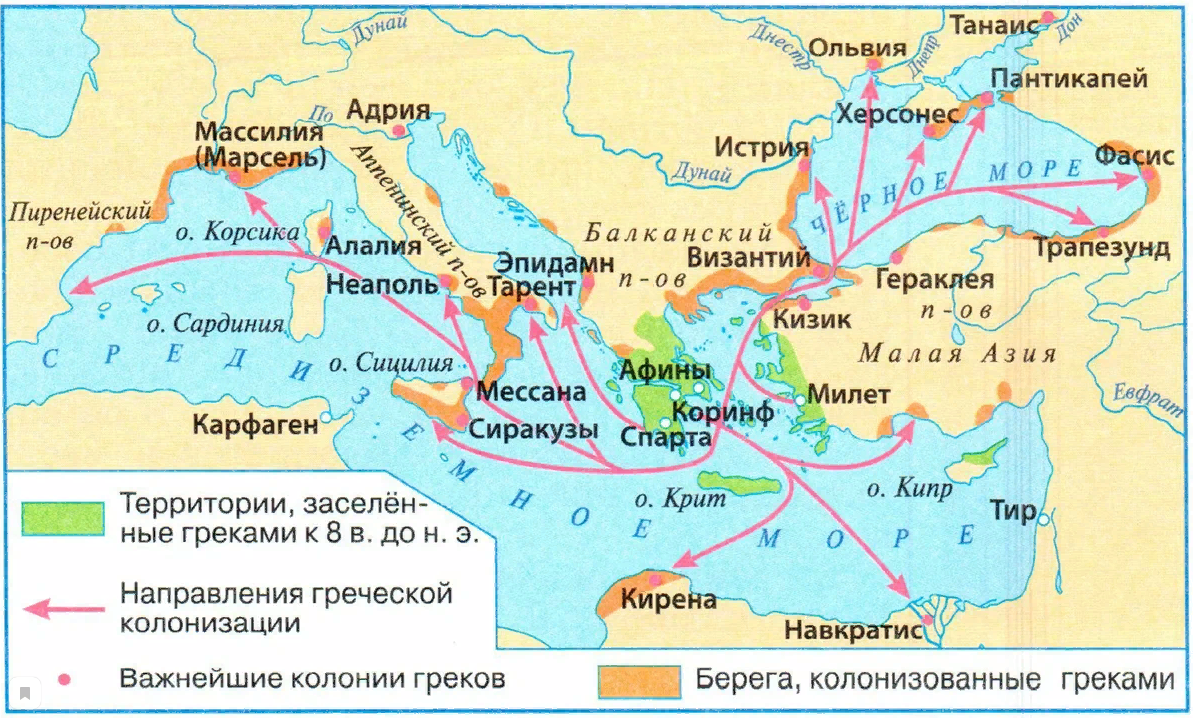
\includegraphics[width=0.5\linewidth]{pictures/greekcolonies.png}
    \label{fig:greekcolonies}
\end{figure}

Древняя Греция не представляла собой единого государства в современной форме. Тогда не существовало привычных межгосударственных границ, а каждый полис фактически представлял собой город-государство, т.к. имел систему управления. Таким образом, межгосударственные отношения выстраивались между полисами. 

% Тогда сформировались политические отношения, тоже от слова полис, отношения
% людей по поводу их совместного проживания, регулирования дел этого сообщества,
% внутренней власти и системы управления. Межгосударственные отношения были
% буквально межполитическими, то есть выстраивались между полисами. И нередко за
% счёт развития дипломатии организовывались союзы таких городов, как для ведения
% междоусобных разборок, так и для противостояния внешним врагам, к примеру,
% персам, стычки с которыми насушенные на море не были редкостью. Внимательно
% посмотрите на карту колоний Древней Греции. 

Важнейшие философские школы были основаны в Милете, Кротоне, Элее, Афинах и других полисах.

\subsubsection{Особенности древнегреческой культуры}

\begin{itemize}
    \item Древние греки были отличными \textbf{мореплавателями} и \textbf{путешественниками}, активно исследовали новые земли, выстраивая с ними экономические и культурные связи за счет обмена товарами и взаимного обучения.
    \item В \textbf{полисах} процветали различные ремесла, торговля, занятия искусствами.
    \item Древние греки высаживались на неосвоенные земли для более удобного осуществления торговли с другими народами, основывая \textbf{колонии}. Т.е. такая колонизация изначально предполагала постройку новых полисов на неосвоенных землях для мирного взаимодействия с другими народами.
    \item На обширных плодородных почвах Средиземного моря развивались оседлое \textbf{земледелие} и скотоводство. \textbf{Рабовладение} для греков было естественно сложившейся и глубоко укорененной в культуре традицией, возникшей первоначально преимущественно по принципу долгового рабства. Примечательно, что во многом именно благодаря рабовладению граждане полиса смогли освободить себе время для обучения, развития наук и искусства, также совершенствования системы государственного управления.
\end{itemize}

\subsubsection{Единство древнегреческой культуры}

\paragraph{Язык}
На древнегреческом языке записывались мифы и легенды, создавались поэтические, эпические, драматические произведения, велась переписка, описывались исторические события, хронология, генеалогия знатных родов, математические расчеты и исследовательские наблюдения.

Открытый доступ общества к произведениям культуры, мифам, истории, наукам, возможность путешествовать, обучаясь в разных местах и древнегреческий язык, интегрирующий все эти формы деятельности, обеспечивали бурное развитие всех сфер культуры Древней Греции. 

Влияние древнегреческого языка на другие языки колоссально. В них используется огромное количество слов, происходящих от древнегреческих корней.
Например:
\begin{itemize}
    \item архэ~---~древний, главный,
    \item атомос~---~неделимый,
    \item феория~---~мысленное созерцание, и т.д.
\end{itemize}

В обыденной и художественной речи используются фразеологические выражения, имеющие древнегреческое происхождение. Например:
\begin{itemize}
    \item Сизифов труд,
    \item Ящик Пандоры,
    \item Ахиллесова пята, и др.
\end{itemize}

\paragraph{Мировоззрение: мифология} 
Единство любой культуры обеспечивается и единством мировоззрения. 
Исторически первой формой представления о мире является мифологическое объяснение его устройства. 

Оно предполагает одушевленный характер всего мира, управления им чьей-то могущественной волей и сверхчеловеческими способностями. Обычно в мифах также предполагается хотя бы случавшийся ранее непосредственный контакт божеств с людьми. 

Мифологические представления удовлетворяли человеческую потребность в объяснении окружающей действительности. Они давали ответы на вопросы о том, как произошел мир, как он устроен, кем управляется, каким нормам и идеалам необходимо соответствовать в собственной жизни.


\subsubsection{Искусство Древней Греции} 
Данные особенности мифологического мировосприятия вместе с вниманием древних
греков к языку не могли не отразиться в искусстве Эллады. 

\begin{itemize}
    \item Для почитания богов строились величественные храмы из камня, в связи с чем развивалась архитектура.
    \item В связи с необходимостью украшения храмов развивались пластические искусства --- скульптуры из камня и бронзы, гончарное мастерство, выкладывание мозаик, а также техника росписи фресками. Изображались прежде всего мифологические персонажи и события с их участием.
    \item Поскольку дела богов мыслились священными и возвышенными, мифы и легенды излагались в поэтической форме (величайшие поэты Гомер и Гесиод), с соблюдением ритма и в сопровождении музыкальных инструментов, постепенно совершенствующихся в связи с этим.
    \item Устная передача мифов и легенд способствовала их значительному искажению, поэтому появилась необходимость письменной фиксации древнегреческой мифологии.
\end{itemize}

\subsubsection{Социокультурные условия}

Распространены празднества в честь богов с фестивалями и обрядами.

\begin{itemize}
    \item Неотъемлемыми элементами праздников являлись театральные представления, разыгрывающие поначалу события мифов и сказания о героях Эллады, а затем и драматические произведения с самостоятельным сюжетом, которые постепенно выделились в отдельный жанр.
    \item Богам посвящались и многочисленные спортивные состязания различного уровня и масштаба (например, Олимпийские игры). Спортивные соревнования, кроме зрелищности, позволяли различным полисам продемонстрировать друг перед другом способности своих атлетов.
    \item Зрелища и праздники, на которые тратились государственные средства, несоизмеримые по своему объёму с другими расходами, на долгие столетия стали единящим древнегреческое общество культурным ядром.
    \item Монархические формы правления архаического периода постепенно сменялись в полисах олигархическими. В правителях полисов ценились прежде всего поступки, а не материальное богатство. Полисы развивались эффективнее под предводительством Совета, учитывавшего социальные и этические потребности граждан, культурно-экономические и военные преимущества.
\end{itemize}

\subparagraph{О популярности трагедий}

В основе их сюжета лежит социально-этическая апория~---~принципиально неразрешимое
противоречие, столкнувшись с которой герой попадает в состояние амехании~---~беспомощности.

Каждый раз героям в конкретике уникальных обстоятельств приходится делать выбор на свой страх и риск. Они мужественно выдерживают распятие на апории, изгоняют в себе пороки, благодаря чудовищным испытаниям судьбы понимают нечто важное, сохраняя человеческое лицо.

Зрители страдали вместе со своими героями и понимали, что настоящее человеческое держится только усилием, стремлением к высшим идеалам и усилием противостояния порокам в себе. Это укрепляло гражданский дух жителей полиса. 

\subparagraph{Об остракизме} Это голосование, в ходе которого каждый член полиса на общем собрании писал на черепке имя наиболее опасного человека для города. <<Победившего>> изгоняли из полиса на срок от 10 лет. 

Практика остракизма побуждала вести себя честно, мужественно, справедливо, сдержанно и рассудительно. Древние греки очень дорожили согласием со своими согражданами, ведь изгнание было страшным позором, а также приводило к потере имущества и социальных связей.

% В Древней Греции средой, через которую каждый отдельный человек приобщался ко всему своему социуму, были массовые празднества, посещение спортивных и театральных зрелищ, а также общение на главной площади города, где в основном обсуждались новости и политические решения, рождались и передавались шутки, сплетни и пр.

Таким образом, к VII веку до н.э. на территориях Древней Греции складываются уникальные по своей специфике социально-культурные условия, способствовавшие выделению в отдельной практике особой формы понимания действительности~---~\textbf{теоретического} мышления. 

\subsection{Феномен <<возникновения>> философии и науки в \\ Древней Греции (в VII-VI вв. до н.э.)}

Говорят о \textbf{\Large<<}возникновении\textbf{\Large>>} философии и науки, так как феномены познания, накопления опыта, передачи знаний, а также такие приемы как обобщение, выделение сущностных связей, классификация и т.д. существовали задолго до Древней Греции. 
Однако это носило фактуальный характер, использовалось исключительно для применения на практике. Свойственное самой природе человека теоретическое мышление не было систематически развиваемо.

В эпоху Античности феномен теоретического мышления отделился от эстетически-мифологического миропонимания. Особенности теоретического уровня осмысления: 
\begin{itemize}
    \item высокая степень абстракции, необходимая для выделения сущностных повторяющихся черт в эмпирическом многообразии явлений;
    \item умозрительный контакт с объектом (независимо от физического ощущения);
    \item обобщение, и др.
\end{itemize}

% VII столетие до н.э. В Древнем Египте, на Месопотамии и на Востоке, в Древней Индии
% и в Древнем Китае известны феномены познания, накопления опыта и передачи
% знания. Однако, если можно в этот период говорить о развитии науки, то это была
% практическая деятельность, а знание было фактуальным, то есть знанием о фактах,
% которые прекращались, прежде всего, в обыденной жизни для тех или иных
% практических нужд. И даже, казалось бы, самая теоретическая наука, математика,
% использовалась исключительно для применения на практике, для счета измерения
% предметов, планирования земельных участков и строительства. 

% Так что, когда говорят о
% теоретическом мышлении античной культуры, надо понимать, что вовсе не имеют в
% виду, что до этого люди не умели обобщать, выделять сущностные причины и явления
% или оперировать теми же числами, как предельной абстракцией. Речь идет о том,
% что 

В Древней Греции к VII веку до н.э. сложился комплекс условий, в которых:
\begin{itemize}
    \item мифологические представления не могли дать ответы на интересующие человека вопросы о том, почему все устроено \textbf{именно так}, зачем человек должен (и должен ли) быть таким, как его рисует миф;
    \item культурная и социально-политическая жизнь побуждала специально развивать и практиковать именно теоретические способности.
\end{itemize}

\paragraph{Причины и основания выделения теоретического мышления}

\begin{itemize}
    \item Сложившийся в рамках мифотворчества соревновательный дух, а также публичность и зрелищность культуры Древней Греции побуждали поэтов, актеров и др. совершенствовать свои умения и навыки. В результате развития словесных речевых жанров активно начали использоваться художественные приёмы: метафоры и \textbf{сравнения}, \textbf{сопоставления}, что требовало и высокого уровня \textbf{абстрагирования} (мысленного одновременного представления нескольких вещей, событий или феноменов и выделения в них на фоне общего особенного).
    \item В силу освоения мореходства и международной торговли происходило активное знакомство с другими этносами и их культурами. Традиции, обычаи и мифологию других народов греки сравнивали со своими, что сказалось на широте кругозора эллинов и переосмыслении собственного привычного уклада и мировоззрения с учетом опыта других народов.
    \item Становление олигархических, а затем демократических режимов правления в полисах приобщало свободных граждан к вопросам правления. Для участия в политической деятельности на собраниях (проводившихся на центральной площади~---~агоре) требовались особые личностные качества, самостоятельность мышления, критический подход, умение рассуждать, аргументировать свое мнение, владение ораторским мастерством.
\end{itemize}

Миф и искусство не давали ответов на многие интересующие человека вопросы (например, из чего все состоит, что такое добро и зло, и др.). Возникла необходимость осмыслять ряд вопросов другими средствами. Умозрение стало основой античного теоретического мышления как метод, с помощью которого можно проникнуть сквозь видимость к истинной сути вещей. Несмотря на это, миф и искусство продолжали выполнять собственные функции.  

% Ни миф, ни искусство сами по себе ответить на подобные вопросы
% были не способны.


% В совокупности с открытым доступом к образованию, что мы тоже уже отмечали, потребность в таком
% типе мышления в огромной степени способствовала развитию дисциплин, логики и
% риторики, а затем и становлению философского подхода. Все эти условия в целом
% дали, как мы бы сейчас сказали, синергетический эффект. То есть совместно
% благотворно повлияли на интенсивное развитие рефлексивного и теоретического
% мышления, чего в условиях других величайших цивилизаций того же исторического
% периода не произошло. Абстрагирование, выделение общего, сравнение,
% сопоставление осуществляется умозрительно, то есть не путем практических
% манипуляций в мире, но способом воссоздания в своем уме общей формы для
% сопоставленных вещей или явлений. 

% Для чего же был выделен и культивирован этот
% специфический способ мыслить? Как мы уже проговорили, мифологическое объяснение
% мира, догматическое, по своей сути, не могло объяснить абсолютно все. Человеку
% свойственно задаваться вопросами и живая тяга к пониманию никогда не уложится ни
% в один статичный конструкт, ни в какие жесткие рамки.   Поэтому древним грекам вовсе не обязательно было отказываться от
% эстетического наслаждения посредством искусства или от мифологического
% объяснения вопросов сотворения Вселенной, влияния на человеческие дела. Просто
% , чем миф или
% искусство. 

\paragraph{О причинах возникновения науки и философии}
Многие исследователи реконструируют \textbf{\Large<<}возникновение\textbf{\Large>>} науки и философии как  появление новых практик в силу неспособности мифа отвечать на интересующие вопросы:
\begin{itemize}
    \item Формула <<от мифа к логосу>> принадлежит советскому антиковеду Ф.Х. Кессиди.
    \item Подобное понимание характерно для и А.Ф. Лосева, исследователя культуры в ее символическом и эстетическом измерениях.
    \item Мераб Константинович Мамардашвили говорит, что наука не появляется из простого накопления техник, умений, но обязательно человеку должно стать что-то непонятно. В мифе все объяснено, и непонятного нет, а проблемность~---~это черта науки.
\end{itemize}

С одной стороны, обильная историческая, философская литература
подводит к такому варианту: первые теоретические произведения появляются с VII-VI веков до н.э (Фалес Милетский, Пифагор и др.).

Но при этом для мифов характерны новые ветки сюжетов, накопление подробностей, добавление уточнений в них при устной передаче. Возможно, если бы люди не задавались вопросами, миф был бы один раз и навсегда.

Это наводит на мысль что, возможно, философию, науку и теоретические понятия не изобрели в этот период, а лишь обратили внимание на вопрошание и осмысление как отдельный вид деятельности.

\subsection{Онтологические основания и сущностные черты античного мировоззрения}

\paragraph{Идеалы и особенности мышления}

\begin{itemize}
    \item Любовь к рассказыванию историй, отражённая в мифах, усиливала интерес к генеалогии. Со временем это привело к поиску \textbf{причинно-следственных связей}, сделав \textbf{рефлексивность} (осмысление через вопросы о причинах) фундаментальной особенностью древнегреческого мышления.
    \item Древние греки интересовались всем~---~от новых земель до древних преданий, от замысловатого движения звезд до отражения окружающих предметов в капле воды. Их культура внимания не выстраивала иерархию вещей: движение далёких звёзд и роса под ногами были одинаково значимы, как и рассказы о богах и размышления о человеке. Первые философы утверждали: \textbf{<<всё во всём>>}~---~всё состоит из \textbf{одного} и может безгранично \textbf{превращаться} друг в друга. Мрамор становится статуей, зерно~---~хлебом, а пища~---~ движением и мыслью.
    \item Греки восхищались совершенством природы и стремились подражать ей в искусстве, создавая \textbf{завершённые цельные} образы. Осознавая изменчивость мира, они умели видеть уникальность и полноту каждой вещи. Целостность, оформленность и границы стали их идеалом. Понимание сущего происходило через видение его \textbf{границ}, его формы, его единичности как завершенности и полноты. Поэтому \textbf{единица} в античной культуре не была просто числом, а основой числового ряда, счета. Важнее всего была целостность предмета, а сам мир воспринимался как упорядоченная, наибольшая единица.
    \item Греки ценили \textbf{упорядоченность} природы, что отразилось в их искусстве и мышлении. Главными принципами стали \textbf{гармония} и \textbf{соразмерность}. Ценность имело целое в единстве своих разнородных частей. Всё соизмерялось~---~от пропорций колонн до тонов в музыке. Раз небесные сферы движутся гармонично, то и человек должен уподобляться им, упорядочивая мысли и организуя жизнь.
\end{itemize}


\paragraph{Онтологические основания античной культуры}

\begin{enumerate}
    \item Как понимается отношение Человек-Мир?

Античный мир представлялся как гармоничный и упорядоченный \textbf{космос}, где каждая единичность была целым. Человек понимался как \textbf{микрокосм}~---~отражение Вселенной в меньшем масштабе, а его жизнь должна была стремиться к той же упорядоченности и соразмерности.

Идеал заключался в совершенстве как внешнем, так и внутреннем. Занятия должны воплощать совершенство, упорядоченность и оформленность мышления, что выражалось понятием Логос. Этическим ориентиром стала добродетель (арете)~---~неотъемлемое качество разумного и правильного человека.


\item Что мыслится несомненным?

Для древних греков несомненным было представление о \textbf{единстве} всего \textbf{сущего}. Несмотря на видимое многообразие, теоретическое мышление позволяло постигать скрытую связь вещей. Если всё превращается друг в друга, значит, существует единое первоначало, из которого состоит всё.

\textbf{Логос}, пронизывающий Вселенную, обеспечивал её порядок и, отражаясь в человеческом разуме, давал возможность и гарантировал способность познавать мир. Это стало основой для теоретического знания, связывающего науку с реальным устройством мира.

Однако античная мысль была разнообразна. Философы спорили о природе материи, причинности, устройстве мира. Поздние школы~---~стоики, эпикурейцы, неоплатоники~---~часто расходились во взглядах. Поэтому вместо <<интуиции Единого>> (А.В. Ахутин) точнее говорить об интуиции Логоса~---~принципа, связывающего всё воедино, но включающего в себя противоположности и парадоксы, которые греки стремились осмыслить.

\item Что значит быть в рамках соответствующего типа мышления?

% По-настоящему быть означало иметь форму, быть целым, завершённым, то
% есть имеющим границы, умеренным и при этом соразмерным остальному порядку мира.
% Категория меры имеет для понимания античного видения ключевую роль. В
% действительности реально быть, быть действовать, значит иметь меру, внутреннюю и
% внешнюю соразмерность. Идеал человека быть живой мерой, то есть каждый раз, в
% каждой уникальной единичной ситуации как бы примеривать себя к ней, соизмерять
% всё и действовать размеренно, умеренно, согласно определённому порядку, а не
% метаться хаотично, беспорядочно действуя и не делать ничего сверх меры. 

Быть по-настоящему~---~значит иметь форму, быть целым и завершённым, соразмерным остальному миру. Ключевую роль в этом играет категория меры. Реальность бытия заключается в внутренней и внешней соразмерности. Идеал человека~---~быть живой мерой, действуя умеренно и согласно порядку, соизмеряя свои действия с каждой ситуацией, а не хаотично и сверх меры.

% Ничего
% сверх меры тоже одна из своеобразных формул древнегреческой культуры. Согласно
% такому пониманию, теперь становится ясно, например, почему богатые представители
% античного общества, обычно к тому же воскообразованные, одевались скромно, не
% пытались чрезмерно украшать свой дом или просто копить свои богатства в виде
% золота. Умеренность во всём означало искусство гармонично упорядочивать свою
% жизнь, цель которой отнюдь не могла быть мысленна в накопительстве или наоборот
% в безмерном расточительстве. Тогда и быть познанным в качестве предмета или
% явления мира означало быть включённым в гармоничное целое миро, быть понятым в
% качестве оформленного и при этом соразмерного с другими элемента. 

«Ничего сверх меры»~---~важная формула древнегреческой культуры. Богатые античные граждане, даже если были образованы, одевались скромно, не излишне украшали дома и не копили золото. Умеренность означала искусство гармонично упорядочивать жизнь, избегая как накопительства, так и расточительства. Быть познанным в мире означало быть частью гармоничного целого, соразмерным с другими элементами.

% Всё беспредельное, а естественно, древним грекам были знакомы математическая
% бесконечность и представления о безмерном мыслились существующими лишь
% возможности. Их можно было вообразить себе, представить. Однако, поскольку в
% мире космосе мы не сталкиваемся с такими вещами, а наоборот наблюдаем
% упорядоченность форм и конечность всего внутримирного, то всему беспредельному,
% неоформленному, аморфному, безразмерному, неумерному и так далее, античный ум
% отказывал в действительном, реальном бытии. Действительное больше возможного. Все наши воображаемые возможности лишь у нас в голове. Они не имеют воплощения в реальности. 

Для древних греков бесконечность и безмерность существовали как абстракции, возможные лишь в воображении. Всё беспредельное, аморфное и неумеренное не имело реального бытия~---~только возможности, которые существуют лишь в воображении. Поэтому действительное считалось большим возможного.

% То есть, смотрите, при всей
% похожести современности на античность, особенно позднюю, что я постараюсь вам
% показать на следующей неделе, основополагающим антологическим различием наших
% эпох является прежде всего разное отношение к категориям возможного и
% действительного. Сегодня нам очевидным и несомненным представляется, что
% возможность больше действительности. Ведь мы можем новоображать кучу всего, что
% может произойти, чего в реальности непосредственно здесь сейчас нет. И на
% основании этого мы поступаем и выстраиваем свою жизнь сплошь и рядом. Например,
% живой классик, итальянский современный философ Пауло Лаверно абсолютно верно
% подмечает, что, скажем, принимая человека на работу, работодатель смотрит не на
% то, что человек реально делает, а доверяет ему, что у того гипотетически есть
% способности для выполнения возможных задач. В свою очередь, работодатель обещает
% сотруднику тоже возможности карьерного роста и определенных премий или повышения
% со временем заработной платы. На деле не факт, что все это оправдается, но мы
% полагаемся на такие воображаемые возможности. В Древней Греции надо было на деле
% показать свое мастерство, чтобы получить признание, уважение и элементарное
% вознаграждение за работу, показать, что ты умеешь, что ты уже реально сделал,
% будь то атлетические спортивные трюки или глиняные горшки, песни или лошадиный
% упряжь. Мы же на каждом шагу думаем, что у нас много возможностей пойти учиться
% туда-то или туда-то, стать тем-то или тем-то, с этим ли человеком сблизиться,
% куда поехать отдыхать, какую одежду для кого-то в случае купить. А что на самом
% деле, каков настоящий выбор в сфере дел, поступков в мире, а не в голове. И эти
% наши воображаемые возможности с удовольствием подпитывают рекламу, пропаганда и
% социальные стереотипы. Мы сегодня очень мало смотрим на то, что действительно
% здесь, сейчас реально есть. Мало всматриваемся в то, какими мы сами на самом
% деле от природы являемся, а не какими нас хотят видеть в этих воображаемых
% стереотипах. И, к сожалению, немало людей проживают в жизни, лишь строя планы в
% голове и представляя себе, что у них есть возможности. На деле же из-за этого
% ничего не успевая по-хорошему воплотить. 



% А что
% реально? Что в мире по-настоящему? Вот это греков интересовало прежде всего.
% Конечно, мы отметили, что они первые начали специально практиковать
% теоретические занятия, которые как раз именно в нашем воображении целиком
% происходят. Но, обратите внимание, для античных исследователей разум
% воспринимался как инструмент. Инструмент осмысления действительности, а не в
% качестве пространства идолов и мечтаний, которым мы отдаёмся в рабство вместо
% жизни в реальности. Безусловно, у человека любой эпохи существует соблазн витать
% в облаках и погрязнуть в мечтаниях, не замечая того, что на самом деле
% происходит. Однако, сами антологические условия, внимание античности к
% настоящему, подлинному, действительному, к природе, как она сама по себе есть и
% к человеку, какие поступки он совершает перед лицом сообщества, побуждали, что
% называется, заняться делом и воплощать, в том числе, прекрасные произведения
% искусства в реальность. Это очень важный момент для понимания всей
% древнегреческо-философской научной мысли, поэтому постарайтесь тщательно
% запомнить такой ключ к эпохе, антологические основания древнегреческой культуры.
% Перейдём теперь в завершение нашего первого вопроса, отталкиваясь от этих самых
% фундаментальных оснований эпохи к гносеологическим, этическим и эстетическим.
% Интересно здесь прежде всего то, что в античности они были фактически
% неразличимы, перетекали друг в друга. Основным источником познания мыслился тот
% самый логос, несомненно, антологический принцип, то, что через всё в мире течёт
% и всё упорядочивает как в космосе, так и в человеке. 

% Логос~---~многозначное
% понятие. Давайте кратенько здесь раскроем спектр его смыслов и отметим его
% логоносеологическое значение для античного способа познания. Во-первых, это
% слово или речь. В этом смысле, например, название науки филологии происходит от
% греческого «любовь к слову». Во-вторых, не теряя своего значения речи, логос,
% как вводилось это понятие первыми древнегреческими философами, мыслился как
% некий всеобщий порядок Вселенной, который пронизывает всё своим течением. Логос
% и однокоренное с ним лего, как конструктор назван, собираю, означает упорядочно
% конструировать. Слушающаяся этого единого порядка природа кампуса образовывает
% своё бытие с всё пронизывающим течением космической речи, делающей мир
% членораздельным, оформленным. В-третьих, под логосом понимается мысль или
% упорядочно оформленное мышление, мышление в понятиях, что на современный манер
% можно трактовать как научную теорию. С данным значением как раз коррелирует
% название дисциплины логики, которая нацелена на обучение правильности
% упорядоченности мыслей и суждения. Сегодня при выяснении темологии название
% большинства научных дисциплин, заканчивающихся на логии, типа биология,
% психология, геология и подобных, логос в соответствии с данным значением так тут
% как учение, что соответствует в частности пифагорейскому оттенку понимания этого
% слова. Так, обучение правильному мышлению, настройка своего ума на слышание,
% видение, текущего через все единого порядка обеспечивало по мнению
% древнегреческих исследователей подключение к логосу как бы программе, которой
% запрограммирована вся вселенная. И тогда всматривайся, анализируй, схватывай
% порядок и придешь к истинному знанию. Так что истинное знание это логично,
% полученное путем умозрительного постижения действительности через рассуждение,
% которое обязательно соотносится с тем, как все реально есть, как мир нам
% является. Поэтому не удивляйтесь, когда мы начнем рассматривать воззрение разных
% античных мыслителей. Они не согласуются друг с другом содержательно. Каждым
% авторам предлагаются разные объяснения причин природных свойств материи. Один
% будет утверждать, что первое вещество, из которого в разных модификациях
% составляются вещи, имеет свойство жидкости, поскольку все течет, изменяется, да
% и без влажной среды нет жизни. Другой будет показывать, что в основе всего
% огонь, как энергия, которая все в разной степени наполняет своим действием. И
% попробуйте на основании современной физики поспорить, что материя в пределе не
% энергия. Третий выскажет предположение о том, что материя в пределе число. И все
% вещества формируются как отражение комбинаций этих чисел, а главное
% соразмерность, гармоничное отношение. И попробуйте, исходя из современных
% квантовых представлений о химической связи, поспорить с тем, что соединение не
% обязано своим существованием как раз гармоничной согласованности энергетических
% уровней, на которых находятся электроны, и которые никак попало образуют связи,
% а в строгой порядоченности по определенным квантовым числам. Ну и так далее. Все
% эти объяснения реально логично выводятся из определенных основоположений,
% которых в рамках своего учения каждый исследователь придерживался. И более того,
% звучат равноубедительно даже для нас сегодняшних, хотя и на непривычном языке
% выражено то, что мы в своих научных теориях сегодня знаем. Это происходит,
% поскольку каждая такая концепция рационально схватывает в действительности то,
% что на самом деле имеет место. Другое дело, что каждый схватывает что-то со
% своего уникального угла зрения, как бы какую-то более близкую грань в изучаемом
% и не может охватить абсолютно все многообразие, выразив в едином
% непротиворечивом принципе. Так что конкуренция познавательных конструктов наших
% теорий одного и того же это нормально в любое время и античность, несмотря на
% стремление к единству и попыткам его схватить выразить, не исключение, а скорее
% первая научная эпоха, которая задает такое правило многогранного рассмотрения. И
% тут, ребята, до меня на новом уровне доходят идеи Артегии Гассета. Помните, на
% прошлой теме я вам цитировала про неизменность истины и изменчивость нашего
% знания на примере формулирования Ньютоном законов всемирного тяготения. У Ганса
% Георга Гадемера, выдающегося современного разработчика философской герминевтики,
% есть подобная идея об истории как истории переосмысления понятий. Мы тоже это
% затрагивали на прошлой неделе по поводу разного смыслового наполнения
% философских категорий в разной эпохе. И вот банальные вроде бы идеи, но я читаю
% античные первоисточники и проводя параллели с современной наукой прямо
% прочувствовала на каком-то качестве на новом уровне для себя. Реально, ребят,
% смысл знания, прозрение человека в сущность мира, порядка вещей вообще не
% меняется. Но язык устаревает, и каждому новому поколению приходится фактически
% изобретать новый язык, более понятный, чем те записи прошлого и трактаты
% древних. Переоткрывается постоянно одно и то же, потому что логично же,
% фундаментально природа не поменялась. Вселенная та же человек, так же
% биологически тысячелетия, десятки тысяч лет назад. Но понятая кем-то и
% выраженная языком его культуры истина может быть непонятна другому, даже
% соотечественнику, скажем, его внуку. Непонятно в силу как раз фиксированности в
% каких-то формулировках, уже не работающих для сознания новых поколений в новых
% условиях. Конечно, существует прогресс как знания, так и мысли, но некоторые
% фундаментальные законы природы и существования человека остаются теми же. Мы
% просто сквозь призму своих социокультурных условий переводим их каждый раз на
% язык более понятных нам мировоззренческих оснований. Вот поэтому, ребята, мы
% изучаем античных авторов. Они уже максимально разработали то мыслительное
% пространство для науки и философии, в котором мы до сих пор движемся, из-за
% границы которого вряд ли человек выйдет, по крайней мере, пока он человек. По
% поводу преобладающих методов познания можно после этого нашего разговора уже
% даже не комментировать. Мы только что проговорили о возможном и действительном
% вонтологических основаниях. Вспомните теперь со второй темой, чем отличается
% наблюдение от эксперимента и соотносите со следующим соображением. Поскольку для
% нас современных важнее и больше кажется возможным, в нашей науке с нового
% времени процветает эксперимент. В отличие от наблюдения, которое происходит в
% естественных условиях, эксперимент создаётся в искусственных. То есть он нацелен
% на раскрытие не того, как природа сама по себе естественного действительности
% есть, а того, какой она может быть, как она может действовать. То есть цель
% раскрытия потенции, возможностей, а не рассмотрения актуальной действительности,
% как в наблюдении. Безусловно, каким бы эмпирическим методом мы не пользовались,
% теоретическое осмысление будет лежать в основании и для античных исследователей
% важно было рационально осмыслить наблюдаемое, сформулировать на логичных
% основаниях красивые, предельно простые обобщённые законы, а не просто
% зафиксировать описание происходящего, что и так испокон веков до них все делали.
% Но самое главное, чтобы вы понимали, я выражу это фразой Анатолия Варьяновича
% Ахутина, грекам показалось бы парадоксальным, если бы кто-нибудь решил изучать
% естественное, то есть природу и естество неестественными методами. В общем-то,
% тоже абсолютно логично. В природе ведь есть только то, что есть, и возникает то,
% что возникает, так наблюдай хорошенько за действительностью и познаешь всё. Ведь
% возможностей в реальности нет, могло бы быть иным, но не иное, вот такое, какое
% есть. И зачем тогда забывать себе голову фантазиями, если мы вот в этом, именно
% в таком действительном мире живём, а не в придуманном. Ну а для современных
% людей это логические условия такие, что им легко впадать в проживание
% ненастоящей жизни, то есть в ненастоящем воображаемом мире возможностей.
% Наконец, в этом свете не менее естественно, что знание развивалось обо всём
% подряд. Нет, наверное, такого феномена или такого объекта, которого бы не
% коснулось этичное любопытство. Так что в эту эпоху было создано знание по всем
% областям действительности, зародились практически все наши современные науки, от
% физики до истории, от биологии до психологии. Особенностью же эпохи является то,
% что не выстраивалась особая иерархия дисциплин, ни в философии, ни в сфере
% научного познания, да и между философией и наукой граница не проводилась. Даже
% попытавшийся аранжировать по степени значимости для человека дисциплины
% Аристотель сам создал головокружительную по своему охвату систему знаний просто
% обо всём и равно был захвачен как подробнейшим наблюдением за животными, так и
% мысленным созерцанием первопричин всего сущего, как пониманием причин
% метеорологических явлений вроде молнии и радуги, так и разбором устройства души.
% То есть, можно, безусловно, говорить особенно про позднюю античность после
% Аристотеля, что намечается ценностное превознесение метафизики, первой
% философии, которая должна прояснять самые фундаментальные первоосновы всего, но
% она важнее, поскольку более фундаментальная. И, как Аристотель говорит, без
% понимания первых причин любое наше знание будет шатким и фрагментарным. И,
% конечно, чтобы упорядоченно мыслить и не совершать ошибок в познании, неплохо
% овладеть инструментарием логики. Однако, это просто вспомогательная, буквально,
% инструментальная дисциплина. Остальные сферы исследования уже отталкиваются от
% определенным образом выстроенной антологической базы, но на которой равна
% строится как этика, так и физика, как медицина, так и политика. Что важнее из
% этих наук? Вот для античных мыслителей было очевидно и несомненно, что все эти
% области одинаково значимы и все их надо развивать. Это дает нам возможность, в
% конце концов, плавно перечечь в этические основания и эстетические идеалы.
% Принципы разумности, гармоничной упорядоченности, соразмерности, это
% одновременно не только антологические принципы, но и этические и эстетические
% идеалы. Страшное слово «калок аготия» обозначает одновременно эстетическую и
% этическую добротность. Происходит от древнегреческого выражения «калос каи
% аготос», буквально «прекрасный и хороший» или «красивый и добрый». Этот принцип
% предполагает совместное обязательное сочетание в человеке физической красоты и
% добродетельности натуры. То есть был даже такой стереотип, если человек некрасив
% внешне, то, скорее всего, он не особо хорош по характеру. Например, Сократа
% завистники порицали за его курносость. Это считалось у греков некрасивым, хотя,
% на мой субъективный взгляд, вполне обычный, непротивный мужчина, тем более с
% отменным здоровьем. Он специально закалялся и регулярно выполнял физические
% упражнения, а в Пелопонесской войне принимал участие в качестве гоплита,
% пехотинца с тяжелым вооружением, которое носить на себе и которым владеть было
% дело исключительных по силе и выносливости воинов. Но своим обидчикам мыслитель
% отвечал, что хотя и не подходит к общепринятым канонам красоты, он изо всех сил
% старался воплотить в своей жизни, по крайней мере, идеал справедливости,
% рассудительности, мужества, внимательности, добродушия и щедрости. Про
% умеренность во всем, как принцип жизни, мы уже проговорили в антологических
% словах, это, я думаю, тоже особо можно не комментировать. Имеется в виду, что
% идеалом античного гражданина было просто при этом опрятно и гармонично
% одеваться, не демонстрировать ни умеренность в расходе средств или питаний, а
% также уделять внимание равно своему физическому и духовному развитию, чтобы во
% всем была пропорциональность чувства, меры и соразмерности, также и эстетический
% идеал, который можно, конечно, выразить как красота в простоте, гармонии и
% естественности. Очень напоминает, кстати, японский принцип ваби-саби, который
% тоже не только эстетический, но и имеет глубокий антологический смысл. Так что
% в, казалось бы, совершенно разных и похожих друг на друга культурах мы находим
% сходные фундаментальные общечеловеческие основания. Про этический рационализм мы
% подробнее обсудим на следующей неделе, когда будем говорить о Сократе и Плутоне.
% Но пускай он тут у вас тоже будет в философских основаниях, означает этот
% принцип буквально следующий. Если я разумом, а рацию одно да не разум, понимаю,
% что такое благо, добро, справедливость, то я принципиально не могу себе
% позволить поступить злым или несправедливым образом. Обратите внимание, знание,
% гносиологическая категория, неразрывно связано с поступком, а это уровень этики.
% Таким образом, подытожим, для античного мышления не характерны разделения таких
% областей, как антология, гносиология, этика и эстетика. Поскольку
% фундаментальным образом в своей основе всё едино, то ум, красота и добротность
% просто разные грани проявления одного бытия. Оно к нам и в каждом человеке
% должно являться полнотой, только если всеми оттенками играет, когда человек и
% тело своё совершенствует, упражняет, и душу развивает, и разум занимает важными
% задачами, рассуждая логично, и поступает по справедливости, по совести. Всё
% красиво и стройно. 

% Но, ребят, напоследок примечанием обращу ваше внимание вот на
% что. Чтобы у вас не создавались идеализированные впечатления об античности, мы
% тут отметили именно идеалы, то есть то, к чему человек стремился. А как вы
% догадываетесь, реальные люди сплошь и рядом далеки от идеала, поэтому, несмотря
% на высокие этические и эстетические принципы, некорректно было бы превозносить
% античность и думать, вот времена-то были, что, мол, все, как на подбор, умные,
% добрые, красивые. Реальные античные люди, многие, естественно, как и наши
% современники, поддавались соблазнам далеко, не все были симпатичны и
% пропорционального телосложения, не всегда могли умерить свой пыл, гордыню,
% злогу, нерезко поступали несправедливо и так далее, как и все обычные люди в
% любую эпоху. 
\end{enumerate}

Не стоит идеализировать античность. Мы говорим об идеалах, к которым стремились люди, но реальные люди часто от них далеки. Хотя в античности были высокие этические и эстетические принципы, многие люди, как и сегодня, поддавались соблазнам, не всегда были красивы, умны или добры, и не всегда могли контролировать свои пороки, как например гордость или несправедливость.

\section{Первые натурфилософские учения античности}

\subsection{Понятие натурфилософии и ее древнегреческая вариация}
Чаще всего под натурфилософией понимается буквально философия природы, т.е.
целостное осмысление природы как общего понятия, через которое возможно объяснение отдельных явлений и познание фундаментальных законов.

Данное определение предполагает, в частности, что познание природы и ее частей
происходит умозрительно, теоретически, философски, в том смысле, что знание о
природе начинается не с практического взаимодействия с отдельными ее областями и
явлениями, а с построения обобщенного представления благодаря созерцанию
целостной сущности данного понятия и философской рефлексии. 

Отдельные явления и области затем изучаются, в том числе эмпирически, в свете такого представления о природе в целом. Так, натурфилософия, как осмысление категории природы, может иметь место в рамках любой культурно-исторической эпохи и находит свои воплощения, например, в метафизике природы нового времени, в стихийном понимании природы мыслителями романтизма XIX века, а также в современных междисциплинарных парадигмах вроде энергетики. 

В нашей дисциплине, \textbf{натурфилософия}~---~это период становления науки, берущий свое начало в древнегреческих учениях о первоосновах и первопричинах мира и заканчивающийся в натурфилософский период в магически-пантеистических представлениях о природе в эпоху Возрождения. 

В этом смысле натурфилософию именно как период развития науки противопоставляют
экспериментальному математическому естественному знанию, оформляющемуся с XVII
столетия и последующему развитию науки, отграничивающей свою специфику от
философской методологии. 

% Помните на прошлой теме в конце мы делили в отечественной трактовке историю науки ее на два крупных периода натурфилософский
% и период научной рациональности. Так вот в целях нашего курса продуктивно именно
% таким способом понимать натурфилософию, поскольку с помощью данного разделения
% удобно обобщить особенности нескольких эпох становления науки. 

Натурфилософский этап развития науки включает в себя специфику научного знания и научного познания в рамках Античности, Средневековья и Возрождения. 

Объединяющими чертами развития науки в данных периодах являются такие особенности, как:

\begin{itemize}
    \item Теоретический, умозрительный подход к познанию. Эмпирические методы были вспомогательными и использовались для уточнения или подтверждения теории.
    \item Философское осмысление природы как целого, без четкого разделения области.
    \item Изоморфность представлений о природе всех вещей вследствие единого основания понимания категории природы. Иначе говоря, в основе любого естественного объекта или явления видится нечто единое, связывающее его со всем остальным в мире. (Изоморфность --- это сходство различных сущностей по форме.)
    \item Метафизическая ориентированность натурфилософского познания, т.е. преобладание проблематики поиска первоначал и первопричин всего сущего.
\end{itemize}

% О ней мы подробно будем говорить на следующей теме, когда будем разбирать труды Аристотеля, это он ввел само понятие метафизики. 

Несмотря на отмеченные сходства, в рамках каждого культурно-историчес-кого типа мышления натурфилософия приобретает и уникальные черты, характерные только для данной эпохи. 

Для античной натурфилософии характерны следующие особенности. 
\begin{enumerate}
\item Как понимается категория природы?

Природа~---~фюзис, т.е. естество. Естественное положение вещей, как оно непосредственно представляется без специфического ракурса рассмотрения и неестественных ограничений.

Аристотелем фюзис противопоставляется техне~---~искусству, специальной деятельности человека, направленной на создание объектов, которых самих по себе в природе не
могло бы возникнуть. (Например, дерево в форме дерева растет само, а мебель из дерева нуждается в искусстве плотника.)

Античная натурфилософия это фактически физика~---~исследование того, что, как и благодаря чему есть само. Ее задача в том, чтобы изучить что и как рождается, в каких видах существует. Поэтому здесь осмысление движения и преобразования всего сущего устройства Вселенной и жизни души~---~вещи одного порядка.

\item Каков основной источник познания природы?

Логос~---~порядок, пронизывающий Вселенную. Согласно Логосу, как в космосе все организовано и движется определенным образом, так и в человеческом разуме (макрокосме) все логично отражено.

Основным источником было разумное созерцание и теоретическое осмысление в его соразмерности самой природе. В этот период формировались различные учения о природе, но каждый мыслитель подвергал их осмыслению и соотнесению собственным видением. 

% Античные физиологи от Фалеса до
% Лукреция умели начинать с начала с самой природы в ее непосредственной открытости
% логическому осмыслению, однако люди, даже в немля упорядоченной вселенской
% текучести речи Логоса могут не понимать ее смысл, по мнению, например,
% Гераклида, пока не обучаться ясности ее слышания и соразмерному ей проясняющему
% рассуждению, в чем, собственно, виделась обучающая функция философии. 

Для античных исследователей не возникала проблема истины, ведь Логос течет через все, поэтому открыты все возможности для познания, и затуманить его может только собственное нежелание человека учиться логичности. 

\item В чем специфика античного метода познания природы? 

Этот метод принято трактовать как теоретический, умозрительный, рациональный, логический, в том смысле, что знание о природе формировалось на основании логически
построенных рассуждений, в рамках которых мыслитель оперировал категориями,
понятиями, выделяя с их помощью сущностные черты изучаемого. 

Основной первичной операцией было \textbf{абстрагирование}, то есть выделение из видимого, наблюдаемого общих закономерностей, свойств, форм. Предельные абстракции~---~число и геометрическое представление, поэтому с ними неизменно переплетаются натурфилософские учения античности. (Но не в свете достижения точности или абсолютности, а скорее математика суть язык Логоса.)

Другая важная мыслительная процедура~--~\textbf{аналогия}. Это сопоставление, уподобление, перенесение характеристик одних объектов на другие.
\end{enumerate}

\subsection{Философская проблема первоначал и первопричин}

\begin{enumerate}
    \item Есть ли у мира начало, или он существовал вечно?
    \item Из чего все состоит? Что собой представляет единая основа всего?
    \item Почему в мире все именно так устроено, как нам является (цвета, звуки, материалы, формы и т.д.)?
\end{enumerate}
Данный спектр вопросов образует собой единое смысловое поле проблематики, которое принято обозначать как <<Проблема первоначал и первопричин мира>>. 

Вопросами, подобными рассмотренным, задаются люди любой эпохи: в этом смысле они являются вечными философскими вопросами. Но в контексте каждой эпохи даются различные по своему содержанию ответы, отражающие онтологические основания того времени.

% К особенностям первых философских сочинений относятся и то, что они в значительной степени не сохранились, дойдя до нас преимущественно в изложении и интерпретации более поздних мыслителей. 

У авторитетных философов естественным образом появлялись ученики и
последователи, которые передавали учения наиболее выдающихся мыслителей. Так
органичным образом складывались \textbf{философские школы}~---~спонтанно возникающие сообщества мыслителей, учеников и последователей, которые разделяли определенную концепцию. 

В отсутствии каких-либо ограничений на
свободу мысли сложилось так, что различные мыслители находили отличающиеся друг
от друга ответы на данный вопрос. Все они были достаточно убедительными,
последовательными, логичными, поэтому даже не совпадающие концепции нельзя
называть ложными или выделить только одну из них в качестве единственной
истинной.

\subsection{Милетская школа философии: вопрос о Первоматерии}

Хронологически первой философской школой Древней Греции является Милетская (полис Милет в Ионии). 

\paragraph{Фалес Милетский}

Это выдающий человек с обширными познаниями в различных сферах, путешественник, получивший образование в процессе странствий и изучения культур других народов. 
Во всех сферах своей жизни Фалес целенаправленно практиковал теоретическое мышление (впервые точно предсказал солнечное затмение, изобрел метод измерения высоты пирамид). 
% Учение Фалеса сохранилось лишь в уцелевших фрагментах его непосредственных учеников и трудах более поздних мыслителей, ссылавшихся на произведения милетцев.

Как философ, Фалес интересен прежде всего постановкой вопроса о первоматерии, из которой все состоит~---~она была названа им \textbf{архэ}. 
% К VII веку до н.э. у многих народов уже сложились не только чисто мифологические представления о мире, но, конечно же, и мнения, выводимые из непосредственно наблюдаемых феноменов, которые мифологизировались. Так достаточно распространенным было представление о четырех, иногда пяти стихиях, материя и движение которых образует все видимое в мире многообразие. Данные стихии огонь, воздух, вода, земля и эфир, как некая высшая спустанция, обожествлялись, с их силами связывались природные и климатические явления, им приписывались сверхъестественные свойства. Но с современной точки зрения это аналоги скорее агрегатных состояний веществ, чем химических элементов, хотя тоже элементами назывались. Важны в этих первостихиях свойства. Например, землистыми считались все твердые тела, с водой отождествляя все жидкости, с воздухом все газообразные тела и так далее. 
В свете интуиции Логоса Фалес предпринял попытку выделить \textit{единое} основание для всего и видел \textbf{воду} в качестве первоматерии. 
Ведь без воды все живое вскоре погибает, при поливе растения дают хороший урожай, моря и реки дают рыбу, все живое сдержит влагу.  Вода представлялась в таком качестве в более широком смысле, как жидкость вообще.  Другие же стихии получаются путем превращения воды.

На основании данного философского учения Фалес логически выводит, что небесные тела не божественные сущности, а состоят из того же самого, но они чрезмерно разогреты, поэтому светятся. Это революционная идея для того времени.

% Безусловно, нам сегодняшнее понимание воды в качестве
% первого начала кажется ложным, потому что мы привязываемся к словам. Для нас
% вода и элемент означают не то же самое, что для древних. Однако обратите
% внимание не на содержание учения, а на метод, на логически выстроенное
% рассуждение. Тогда становится понятно, что в свете обозначенного нами духа эпохи
% и ее антологических оснований из повседневных наблюдений достаточно естественно
% было придать именно чему-то жидкому, зримо присутствующему повсеместно, статус
% материального, текучего, изменчивого основания мира, из которого все состоит.


\paragraph{Анаксимандр} Ученик Фалеса Милетского.
Многое сделал, чтобы язык философии отделился от художественного стиля изложения в стихах, а содержание было достаточно самостоятельным от мифа. В частности, он писал свои труды в прозе. 

Наблюдая превращение друг в друга четырех стихий, Анаксимандр не счел возможным взять
одну из них за основание, и принял за него нечто от них отличное. Первоначалом мыслитель считал \textbf{апейрон} (беспредельное):

Анаксимандр считал, что свете вопроса о первичности мера оказывается вторичной, ведь она ограничивает, а это необходимо делать с уже чем-то имеющимся. 
Значит, если ставится вопрос о первоначале, то оно должно иметь свойство \textbf{неограниченности}, чтобы посредством соединения с мерой дать уже ощущаемые оформленные вещи. Также свою первую материю мыслитель наделяет свойствами \textbf{неуничтожимости} и \textbf{всеобъемлемости}.

Другие достижения Анаксимандра:

\begin{itemize}
    \item \textit{Идея о движущей силе противоположностей}. Вечное движение более древнее начало, чем влага; благодаря ему одно рождается, а другое погибает. Из единого выделяются соединенные в нем противоположности.  Рождение происходит не через изменение стихии, а через обособление благодаря вечному движению противоположностей (например, добро и зло, предельное и беспредельное). Они влияют друг на друга, своим неравенством запуская движение.
    \item Первая формулировка \textit{закона сохранения материи}. Из чего все вещи получают свое рождение, в то все они и возвращаются, следуя необходимости. Все они в свое время наказывают друг друга за несправедливость (занимание собой всего пространства).
    \item \textit{О происхождении человека}. Первый человек произошел от живых существ другого вида, а жизнь вообще родилась в океане, из которого со временем на сушу вышли существа, покрытые чешуей. Их чешуя лопнула, и вскоре они изменили свой образ жизни.
    \item А также начертил первую \textit{географическую карту} мира, занимался вычислениями движения небесных тел, предложил впервые небесный глобус, изобрел \textit{гномон} для усовершенствования солнечных часов и пр.
\end{itemize}

\paragraph{Анаксимен} Ученик Анаксимандра. Свел все причины вещей к беспредельному
воздуху. Он наделил архэ свойствами газообразных тел или стихии воздуха, который как бы вдыхает жизнь во все.  

Анаксимен полагал, что из беспредельного воздуха при разряжении рождается огонь, а при сгущении ветер, туман, вода, земля, камень. Данные воззрения позволяли наглядно представить смену агрегатных состояний и превращение вещей друг в друга.

\subsection{Пифагорейская школа философии: музыка небесных сфер}

Одна из самых многочисленных и влиятельных школ Древней Греции, возникшая в южно-италийском полисе Кротон. 

\paragraph{Пифагор} Уроженец острова Самос в Ионии, обучался в Египте; историки полагают, что Пифагор учился у известного мудреца пророка Зороастра (Заратустры).

% Мудрый дальновидный человек,
% разбиравшийся в людях, умевший убеждать и принимать грамотные политические
% решения. 

% За такие способности италийцы верили пифагору и его ученикам управления
% полисом. 

Учение Пифагора при его жизни оставалось внутри сообщества учеников, связанных обетом молчания. Однако политическая активность пифагорейцев способствовала распространению славы их школы по Элладе.

Сообщество отличалось общностью имущества, а учеников Пифагор отбирал лично. Обучались у него как мужчины, так и женщины. Сочинений самого Пифагора не сохранилось, но дошли отрывки трудов его последователей, в которых излагались основные положения учения
мыслителя. 

% Одному картонцу Келону было отказано вступить в ряд пифагорейцев по
% причине его тиранического нрава. Тогда тот устроил заговор. Собственники Келона
% подожгли здание, в котором заседали пифагорейцы. Выбраться во время пожара
% удалось лишь двоим самым молодым и сильным ученикам, которые покинули Италию и
% поселились на Пелопонесе, решив передавать новым последователям великое учение
% пифагора и опубликовать труды. 

% Размышляя над распространенным тогда пониманием первоначал, как
% соединение предела и беспредельного, Пифагор не только был захвачен присутствием
% других противоположностей во всем правое и левое, мужское и женское, четное и
% нечетное, доброе и зло и так далее, но и уловил присутствие единого в основании
% этих пар. Если бы не было одного основания до всех противоположностей, основания
% фундаментального порядка, согласно которому в мире уже есть разделение, то есть
% мы уже сталкиваемся и имеем дело с теми симметричностями, то противоположности
% нивелировали бы друг друга, аннигилировали или смешали бы в неразличимую массу.
% То есть  Поняв смысл
% поразительной и непостижимой для человеческого ума задумки природы или
% мироздания или высшего разума или Бога назвать как угодно, 

Размышляя о первоначалах как сочетании предела и беспредельного, Пифагор заметил присутствие противоположностей во всем~---~правое и левое, мужское и женское, и т.д. Однако он уловил и их единое основание. Без этого фундамента противоположности либо нивелировали бы друг друга, либо смешались в неразличимую массу. Если бы противоположности и только они были первичны, то это противоречило бы интуиции единого Логоса; кроме того неясно, что удерживало бы их от смешения и взаимного уничтожения.

% Пифагор первым назвал
% себя философом, а не мудрецом. Пифагор таким образом имел в виду, что человек,
% как конечное существо, не может постичь, что предельное основание, благодаря
% которому всё существует, потому что оно до нас, не нами создано и не наравне с
% нами существует. Его не найти в мире, не схватить своим умом, поэтому он
% говорил, что никто не мудр, кроме Бога. Того же, кто желает возвысить свою душу
% и стремиться к предельно ясному осмыслению, подобает называть философом, любящим
% мудрость или другом мудрости. Слово философия от греческого филия любовь и софия
% мудрость на русский язык переводится как любовь к мудрости, буквально
% любомудрия. Это любовь к вселенской мудрости, к софии мира, к тому, благодаря
% чему всё именно так устроено. 

Пифагор первым назвал себя философом, а не мудрецом, подчеркивая, что человек не способен постичь предельное основание бытия, поскольку оно выше и не создано им. Он считал, что мудр только Бог, а стремящихся к истине следует называть философами~---~любящими мудрость. Философия, происходя от греческих слов <<филия>> (любовь) и <<софия>> (мудрость), означает любовь к вселенской мудрости и устройству мира.

% По этому поводу замечательный отечественный
% мыслитель Владимир Вениаминович Бибихин пишет, что смысл пифагорейского учения в
% указании на непостижимый ум, той основы, на которой возникают пары. Когда мы
% приходим в мир, то видим сразу правое, левое и другие пары. Увидеть то единое,
% которым они выброшены, мы никогда не успеваем принципиально. Пифагорейские пары
% указания на нередуцируемую удовольствие на сначала. Нередуцируемую не потому,
% что не к чему больше сводить, а потому, что основа пар не наша София. Мы не
% знаем и никогда не будем знать, какой Софии создан и почему именно эти, а не
% другие морские звезды, которые можно видеть в зоологическом музее. Пифагор ввел
% слово философия потому именно, что говорил о Филии, верности такой Софии,
% которая другого приобщения к себе, никакой причастности к себе не допускает.
% Недоступна эта София, и можно только догадаться об этом и любить ее. Что же это
% принципиально меняет? Казалось бы, какая разница, как называть исследователей
% первооснов и первопричин мудрец или любящий Софию мудрость, а разница
% колоссальная. Представьте себе мудреца, сегодня ведь тоже некоторые люди не
% перестают себя выдавать за мудрецов, такой просвещенный говорит, что познал все
% законы Вселенной, что в мире 42 ступени различных сущностей, человек это только
% четвертое снизу, и надо совершить семь шагов очищения для разных шести типов
% людей, но вы поняли, все расписано и посчитано, и нельзя ставить под вопрос. Вот
% меня, как философа, всегда такие мудрецы, имеющие, дескать, высшее просветленное
% знание, настораживают. Почему? Потому что по определению смертный не может иметь
% абсолютно правильного знания обо всем, да и знание о таких предельных вещах
% невозможно, не потому что у нас не хватает ума техник напридумывать, но потому
% что все эти схемы закрывают собственно человеческое раз и навсегда что-то
% определенное о мире и человеке решить, установить, зафиксировать, а наше дело
% другое. Во-первых, мир не обязан подстраиваться под наши воображаемые конструкты
% и всегда может произойти что-то, что наша схема не описывает. А во-вторых, мы
% сами вопрошающие существа и открытые. На каком основании кто-то решает, что все
% именно так, что бытие представляет из себя то-то и то-то, как смертные могут
% решать, какими быть миру, человеку, чем-то превосходящему нас, предшествующему
% нашему рождению. Наш ум, я уже выше говорила, не случайно с нюхом воздуха
% математологически связан, а душа с дыханием. Закрывая всю повнуту и все
% спонтанное многообразие реальности своими схемами и техниками, такие вот мудрецы
% буквально перекрывают душе воздух, дыхание. И в нагромождении их однозначных
% объяснений нам становится скучно. Мы задыхаемся, потому что никогда по-честному
% не сможем жить в этих закупоренных домиках. Мы ведь творческие существа, а
% значит такие, которым обязательно надо новое. Наконец, честнее оставить
% открытыми вопросы о том, например, есть ли Бог, неужели мы ему можем указывать,
% быть ему или не быть. Возник ли мир или существует вечно? Ведь мы уже упустили
% момент начала, родились уже в мире. Что такое материя? А попробуйте ее
% определить, если она обладает свойством беспредельности. Если мы не знаем о
% таких вещах, может быть, пока не знаем, но вот здесь и сейчас не можем взять и с
% наскоку ответить на подобный вопрос. Так давайте, по крайней мере, достойно
% поступим, по-честному, сохраним лицо, как настоящие исследователи и мужественно
% продолжим держать эти вопросы открытыми. Не спешить впасть в непродуктивные
% схемы, повязывающие по рукам и ногам нашу творческую энергию. Так вот, в каком
% состоянии дышится свободно? В каком мы счастливы? Не в таком, когда у нас есть
% стройное и подробное знание ведания обо всем. А вот любящий не знает, знать и
% ведать не пытается, он видит, принимает и понимает. Свободен и открыт, счастлив
% в состоянии любви. Ведь что же такое любовь, если не абсолютно доверие и
% принятие? Тогда философия принимает все, как оно есть, доверяет устройству мира
% и в своем восхищении продуманностью вселенского порядка смиряется с тем, чтобы
% фундаментальным образом не знать, как и почему все на самом деле именно так. Мы
% любим, например, конкретного человека не потому, что знаем все о нем. Наоборот,
% доскональное знание обо всех подробностях его существования скорее будет мешать
% его любить. Незнание здесь также имеется в виду не в негативном смысле
% необразованности, но в хорошем смысле необязательности модели, конструкции,
% прописанной схемы для любимого, принимаемого, видимого. Ведь любим, принимаем,
% видим мы не схемы и конструкты, а что-то принципиально не нами созданное, что-то
% настоящее, открытое, живое за ними. Хотя без конструкции мы тоже вряд ли можем
% обойтись. Другое дело, надо понимать, для чего они нам служат, и каково должно
% быть их место в нашей жизни. Но любовь, возможно, только к целому, которая
% выбирает в себя парадоксальным образом противоположности в смеси хорошего,
% плохого и нас, и мира. Это, безусловно, не значит, что надо заострять внимание
% на плохой стороне. Мужество настоящей любви заключается в свободе. Дать
% любимому, как конкретному человеку, так и всему миру, быть себе в своей свободе.
% А это означает доверить Софии мира, мудрому устройству, чтобы любимое было само
% собой устроено, без нашего вмешательства. Тогда мы любим, например, вот этого
% конкретного человека, принимаем его полностью, без желания исправить,
% переделать, улучшить, залезть в его устройство и контролировать. Наша свобода в
% том, чтобы делать свое, показывать пример, тянуться к хорошей стороне, хотя она
% не обеспечена, всегда есть и плохая, причем в каждом из нас и то и другое
% вложено, независимо от нашего желания. Это удивительно, замечая это все,
% парадоксальности и полноте нам дано к такому двигателю из двух неравных половин
% фундаментальной парадоксальности всего попробовать как-то аккуратно для
% понимания подключаться.

Смысл пифагорейского учения, по В.В. Бибихину, заключается в указании на непостижимую основу, из которой возникают противоположности. Мы видим мир уже разделенным на пары, но их единое основание остается недоступным. Пифагор назвал себя философом, потому что философия~---~это не обладание мудростью, а любовь и верность ей, осознание ее недоступности.

Разница между мудрецом и философом принципиальна. Мудрецы претендуют на абсолютное знание, создавая жесткие схемы, но мир не обязан им соответствовать. Истинный философ понимает ограниченность человеческого ума, оставляет вопросы открытыми и не спешит фиксировать окончательные ответы. Человеку необходима свобода мысли, а жесткие конструкции перекрывают ему <<воздух>>.

Любовь, как и философия,~---~это доверие и принятие. Мы любим не из-за знания всех деталей, а вопреки им, ценя целостность и парадоксальность мира. Истинная свобода~---~это позволить вещам и людям быть самими собой, без стремления переделать или подчинить их. Философия учит не контролировать, а восхищаться гармонией вселенной, сохраняя открытость перед ее тайнами.

% Вот Пифагор, видимо, был первым исследителем, который
% это четко прояснил. Но подождите, что же в науке ученые не любят? В том-то и
% дело, в этом мы все едины. Настоящий исследователь любит свою научную область,
% ее методологию, свой предмет изучения. Иначе бы не разговаривал со своими
% образцами и приборами, не чувствовал бы их мельчайшего ненастроенность на основе
% цели исследования, не сопереживал бы своим респондентам, читая анкеты, не
% удивился бы красоте формул, методов, языка. Ученый любит процесс познания, он
% захвачен, ему интересно, иначе исследование не настоящее. И его результат в виде
% готового знания. Но обратите внимание, в науке мы как бы пользуемся этим
% продуктивным состоянием, этим позитивным настроем, чтобы делать свое
% исследование. Само наше состояние при этом мы не делаем предметом, мы в его
% свете что-то начинаем видеть, понимать и фиксировать в качестве знания.
% Философия же, в отличие от науки, можно сказать, наоборот, делает своим
% предметом то, благодаря чему оглядывается на само это состояние нашей
% человеческой захваченности. Философия угадывает, что состояние нужно
% настраивать. И будучи любовью к порядку Софии, призвана нам о таком состоянии
% напоминать. 

% Пифагор был также ученым, на разумных основаниях он старался
% создать знания о том, о чем оно нам доступно по поводу природы. Каким же единым
% образом можно понять первоосновы всего в мире? Философ видел
% двоичность предела и беспредельного и понимал логическую невозможность
% отождествить одну из стихий с единой первоосновы. Она единая во всех вещах,
% похож всепронизывающий порядок Софии или в форме какого-то основы. 

%Тогда на что?
% Доступного языка логость течет через наш ум. Ответ Пифагора гениален. Это число.
% Число то, что доступно нашему познанию в единой основе всех вещей. Число это предельная абстракция, на которую способен наш разум. Выделяя в обобщающем мышлении одинаковость формы предметов, мы
% становимся способны их считать. Так, в пределе мы в нашем уме можем оперировать
% числами уже независимо от вещественных коррелятов, то есть математически,
% абсолютно абстрактно. То же самое с геометрическими формами. Когда-то поняв
% сущность, например, треугольника, мы представляем его в своем уме независимо от
% треугольного предмета, а также от того, на бумаге начерчен треугольник, на доске
% или на песке. Мы мыслим и в уме оперируем самой идеей фигуры с тремя углами. В
% связи с этой способностью нашего теоретического мышления пифагорейское учение и
% постулирует число в качестве фундаментальной основы. И число в нашем уме реально
% настолько отдельно от вещей мира, что похоже на отдельность единого логоса от
% всего доступного нам в империи на опыте. Чувствуете, как близко друг с другом
% идут настоящая философия и наука. Благодаря такой аналогии, такому исходному
% пункту пифагорейского учения мы обязаны мыслителям данной философской школы
% прежде всего развитие математики, строящейся вокруг философских проблем предела
% и беспредельного пропорции и отношения подобия и различия форм. Но, естественно,
% в свете сказанного пифагорейское учение о числах и геометрических
% преобразованиях нельзя понимать, как отвлеченное построение математического
% аппарата. Инструментарий этот изобретался и совершенствовался именно благодаря
% своей укорененности в философских вопросах о том, как, согласно с какими
% принципами и законами все в мире устроено. То есть, не сама по себе математика
% была важна, а ее возможности для понимания вселенского порядка логоса, в
% соответствии с которым вспоминаете античные антологические основания устроена
% как космическая гармония, так и земная, как большое, так и малое. Математика
% помогала понять соотношение всего со всем, становилась как бы посредником,
% связующим звеном между всеми структурами мира, то есть, своеобразным языком
% вселенского порядка. Поэтому, занимаясь математическими абстракциями и, казалось
% бы, чисто теоретическими проблемами бесконечной делимости или несоизмеримости
% некоторых чисел, античные мыслители на самом деле с одной стороны настраивали
% свой ум на чистое восприятие форм, а с другой были захвачены самыми
% фундаментальными вопросами нашего бытия и познания, оперируя ими в
% математических терминах. В связи с таким особым статусом математики различные
% числа и геометрические формы наделялись специфическими свойствами, которые
% кажутся непонятными нашему сегодняшнему их восприятию как ценностно одинаково да
% и вообще никак не нагруженных человеческим отношением к ним. 

Пифагор был не только философом, но и ученым, стремившимся к разумному познанию природы. Он видел двоичность предела и беспредельного, понимая, что ни одна из стихий не может быть единой первоосновой. Ответ Пифагора гениален: основой всего является \textbf{число}.

Число~---~это предельная абстракция, доступная нашему разуму. Оперируя числами, мы постигаем единство вещей, а математическое мышление позволяет нам мыслить формы независимо от их материальных носителей. Именно поэтому пифагорейцы считали число фундаментом мироздания.

Благодаря философским вопросам о пределе, пропорции и гармонии пифагорейцы внесли огромный вклад в развитие \textbf{математики}. Однако для них она не была просто инструментом вычислений, а способом понять вселенский порядок~---~Логос. Математика становилась языком мироздания, посредником между структурами мира, позволяя настраивать ум на восприятие космической гармонии. В этом слиянии науки и философии зарождалась традиция постижения бытия через абстрактные формы, что отличает античное мышление от современного утилитарного подхода к числам.

% Единица не выделялась как непосредственно число. Она была началом и основанием любого счета, поскольку для того, чтобы начать считать предметы, необходимо выделить каждый в
% качестве отдельной единицы. идеал завершенности, полноты, оформленности как раз
% соответствует такому ценностному преобладанию единицы как некой самостоятельной
% целостности. Неважно какого размера и космос единица как целая, и каждый
% отдельный человек единица как завершенность, и каждая отдельная капелька воды.
% как пишет один из наших выдающихся философов и историков науки Анатолий
% Вальянович Охотин, единицы таким образом для пифагорейцев разновидны и
% разнокачественны. Если в области зримых предметов происходит деление единицы, то
% она как тело уменьшается и разделяется на меньшие части, но в числовом отношении
% она увеличивается, так как место одной вещи занимает теперь несколько вещей.

Единица у пифагорейцев не выделялась как непосредственно число, а была началом и основанием счета. Чтобы считать предметы, нужно сначала выделить их как отдельные единицы. Единица символизировала завершенность и целостность~---~будь то космос, человек или капля воды.

Как отмечает философ А. В. Охотин, единицы у пифагорейцев были разными по природе. В материальном мире деление единицы уменьшает ее как тело, но в числовом смысле она увеличивается, так как одна вещь превращается в несколько. Таким образом, пифагорейская концепция единицы сочетала в себе идею целостности и множественности одновременно.

% Помимо единицы ценностно нагружались пифагорейцами и другие числа, в частности,
% они полагали число 10 божественным и совершенным, поскольку его составляла сумма
% первых четырех цифр 1 плюс 2 плюс 3 плюс 4, она содержала поровну и четных и
% нечетных чисел, в конце концов десятками нам от природы видимо удобно считать,
% потому что на руках 10 пальцев отсюда пошла наша наиболее распространенная
% десятичная система исчисления, хотя вы, наверное, в курсе, что существуют
% современные математики и множество других, к примеру, на двоичной построен
% принцип действия современных компьютеров. У пифагорейцев числа также
% соотносились с геометрическими формами. Единица точка единая целостная, двойка
% линия, тройка треугольник, как первая плоская фигура, символизирующая плоскость
% вообще, четверка тетраэдр, как первая объемная фигура, символизирующая,
% соответственно, трехмерное пространство. По счету углов и ребер геометрических
% фигур выводятся все их арифметические характеристики. Равенство сторон,
% пропорциональность и симметричность форм мыслятся принципами наивысшего
% совершенства. Чем более правильна и проста фигура, тем она божественнее и
% прекраснее. Что же может быть идеальнее окружности и сферы? Риторический вопрос.

Пифагорейцы наделяли числа особым смыслом. Число 10 считалось божественным и совершенным, так как представляло собой сумму первых четырех чисел (1 + 2 + 3 + 4) и включало поровну четных и нечетных значений. Кроме того, десятками удобно считать из-за 10 пальцев на руках, что предопределило распространенность десятичной системы.

Числа у пифагорейцев также соотносились с геометрическими формами: единица~---~точка, двойка~---~линия, тройка~---~треугольник как первая плоская фигура, четверка~---~тетраэдр как первая объемная фигура, символизирующая трехмерное пространство. Пропорции, симметрия и правильность форм считались высшим проявлением гармонии. Идеалом же совершенства была окружность и сфера~---~фигуры, в которых воплощена абсолютная симметрия.

% Поэтому и космос как наиболее совершенное мыслился сферическим, замкнутым, а
% движение небесных тел представлялось круговым. Математические исследования
% пифагорейцев не были абсолютно умозрительными, находя применение, например, для
% описания космоса и для составления теории музыки. Именно пифагорейцам
% принадлежит открытие и математическое описание музыкальной гармонии на основании
% идеальных числовых пропорций, соотношений. Кто обучался музыке, поймет. Музыка
% во многом математика, поскольку для благозвучности необходим точный расчет
% интервалов и соотношений высот одновременно извлекаемых звуков. Пифагорейцы
% создали основу всей современной теории музыки, исследуя звуки струн, натянутых с
% помощью различных грузов, которые в свою очередь пропорционально относились друг
% к другу по массе один к двум, два к трём и так далее. Кому интересно подробнее
% узнать об этом, почитайте сами, а мы тут подытожим. Поиск пропорций и подобия во
% всём характеризуют методологическую направленность пифагорейской школы, гармония
% и соотношение. Были интересны этим исследователям во всём, от звучания
% музыкального инструмента до устройства Вселенной. Поэтому в заглавии данного
% пункта плана я употребила выражение «музыка небесных сфер» отнюдь не
% метафорически. Земная музыка для пифагорейцев была способом воспроизводить идеал
% космической гармонии, поскольку в своей совершенной упорядоченности космос
% буквально так же звучал, как звучат музыкальные инструменты. 

Поэтому космос, как наиболее совершенное, мыслился сферическим и замкнутым, а движение небесных тел~---~круговым. Математические исследования пифагорейцев не были чисто умозрительными, находя применение, например, в описании космоса и создании теории музыки.

Именно пифагорейцы открыли и математически описали музыкальную \textbf{гармонию} на основе числовых пропорций. Музыка, по сути, математика, так как ее благозвучность зависит от точных расчетов интервалов и высот звуков. Они исследовали звучание струн, натянутых с разными грузами, массы которых находились в пропорциях 1:2, 2:3 и так далее, заложив основу современной теории музыки.

Поиск пропорций и подобия во всем характеризовал пифагорейский метод: от устройства Вселенной до музыки. Отсюда и выражение «музыка небесных сфер»~---~для пифагорейцев оно не было метафорой. Земная музыка воспроизводила идеал космической гармонии, ведь, согласно их учению, сам космос звучал, подобно музыкальному инструменту.

\paragraph{Алкмеон Кротонский} 
Был известным врачом-пифагорейцем, который развил учения о противоположностях применительно к человеческому телу. Он считал, что равновесие сохраняет здоровье, ибо господство одной противоположности действует гибелью (например, как избыток пищи, так и её недостаток вредны для здоровья).

% То же самое с теплом, холодом, духовным и
% физическим развитием и так далее. Это другой взгляд на медицину. В античности
% врач-целитель от слова целое, то есть тот, кто помогает человеку быть целым,
% целостным, а это как нельзя лучше достигается путём соблюдения баланса и
% разумного самоограничения. И действительно, по природе тело стремится к
% здоровью, надо только ему не мешать, в том числе стараться, чтобы связанная с
% ним душа не тревожилась чрезмерно и с другой стороны не изнеживалась.

Алкмеон впервые предпринял препарирование человеческого тела. Благодаря
этому он описал, например, как глаза соединены с мозгом зрительными нервами, чем доказал в частности, что ощущения поступают в мозг через органы чувств, а в целом~---~то, что первенствующая часть души находится в мозге. 

Алкмеон также сформулировал фундаментальное отличие человека от других живых существ: только он, человек, понимает, а другие животные ощущают, но не понимают. 

\paragraph{Филолай}  Впервые опубликовал основы пифагорейского учения, которое до этого было тайным и систематически не распространялось. 

Филолай интересен тем, что как раз, что благодаря сохранившимся его произведениям мы много знаем о пифагорейской философской системе видения мира с помощью языка чисел и геометрических представлений, а также о пифагорейской теории музыки. 

Филолай понимает устройство космоса не геоцентрически, не гелиоцентрически, а как Вселенную, в центре которой находится очаг, вокруг которого вращаются и
звёзды, и Солнце, и другие планеты, в том числе Земля. 

% Вообще я поражаюсь глубине античной мысли, когда, например, читаю у Филолая, что космос питается испарениями вылившихся светил, чем не испаряющиеся чёрные дыры современных астрономов. 

\paragraph{Мнение лектора}
Когда смеются над воззрениями древних греков и считают их зачатками науки, значит, не понимают, насколько наши сегодняшние научные представления повторяют сказанные античными мыслителями. 

Вроде бы смешно считать, что всё есть число или всё состоит из некой единой первоматерии, но давайте присмотримся на вопрос, из чего всё состоит и вдумаемся.  Наши современники отвечают, что из молекул и атомов, а специалисты уточняют из энергии, потому что современная физика выяснила, материя на микроуровне энергия. Те самые элементарные частицы, из которых всё состоит, в пределе представляют собой энергетические уровни или энергетические состояния. 

А что такое энергетические уровни? Это числа, решение уравнения Шрёдингера для волновой функции, значит, материя в пределе число. Но постойте, об этом с конца VI века до н.э. говорят пифагорейцы и вслед за ними Платон. 

Берём примерно более высоком уровне организации материи, если нас сами элементарные частицы не удовлетворяют. Образ любого живого существа с определенными особенностями передаётся от родителей детям, как с помощью генетического кода. А код это шифр, последовательность, которая тоже число или числовой ряд. Так что мы с вами как ни крути, тоже в пределе число. 

Другой пример современной физики. Теория струн очень напоминает пифагорейские струны с их пропорциями. 

\paragraph{Мнение автора} Я не знаю, из чего все состоит :(

% В общем, советую задуматься над таким современным стереотипом, что наука ступенчато развивается, и в каждую новую эпоху знания становятся всё точнее, лучше, правильнее. Мне кажется, реальные люди в каждую эпоху не садятся с грустью дожидаться, пока же наконец пройдём мы современные со своими новыми теориями и техниками. Они сами стараются всё исследовать и понять, сами формируют свою понятную им картину мира. 

% Это нам сегодняшним могут быть непонятны античные первоисточники, если мы не настроились увидеть смысл в них вложенный глазами оснований этой эпохи. На деле далеко ли мы сегодняшние ушли от античных мыслей? В начале предыдущей пары я неслучайно говорила, что вся наука, в том числе сегодняшнее свернуто в идеях древнегреческих мыслителей. Может быть действительно историчность языка описания просто создаёт видимость прогресса? 

\subsection{Гераклит Эфесский: правящая молния}

Гераклит взял на себя миссию критиковать нелогичное мышление и обличать невежество своих сограждан, поддающихся стереотипам. Он был человеком резким и эмоциональным, а его взгляды отличались глубиной и оригинальностью. Современники отмечали его знатное происхождение, а сам он много путешествовал и исследовал мир. В отличие от других философов, Гераклит не учился у наставников~---~всю свою мудрость он постиг самостоятельно.

% В Эфесе к власти пришёл тиран и изгнал из города друга Гераклита Гермодора. Мыслитель призывал граждан препятствовать этому, но они не стали сопротивляться. Когда же потом в спорной ситуации к нему играющему с детьми у храма Артемида прибежала взволнованная
% толпа сограждан и попросила дать им новые законы, Гераклит остался играть с
% детьми, сославшись на то, что город уже во власти дурного государственного
% устройства. Афиняне приглашали мыслителя поселиться у них после того, как эфесцы
% разобиделись на своего философа за подобное поведение, но он предпочёл остаться
% на родине. 

% Даже персидский царь к нему и его друзьям пожелал приобщиться к
% мудрости Гераклита и приглашал его переселиться в Персию под свою опеку.
% Гераклит себя и с царём держал на равных, переписывался с ним, сохранились
% несколько их писем, сообщал о своих идеях царю, но от приглашения отказался,
% слишком был свободолюбив. 

% Гераклит не основал своей школы, от его философии до
% нас дошло всего 139 фрагментов, в основном афоризмы, но чуть ли не во всех
% последующих учениях можно проследить влияние его мысли. Например, Гегель как-то
% сказал «нет положения Гераклита, которое я не принял в свою логику». 

% Гераклит назвал то самое единое начало Логоса и полагал, что этому первичному похожему на речь порядку подчиняются и боги. Логос один и тот же во всём и для всего. 

% Не уступая Пифагору в глубине философской мысли, Гераклит говорил, что мудрость
% София, которой всё устроено отдельно от мира и настолько иная, что мы себе не
% можем её представить. Видим только уже отражение противоположностей в нашей
% Вселенной, их движение, их игру. Другое всему отдельное это та половина
% Гераклитовской мысли, о которой Сократ сказал, что он её не понял. Чтобы понять,
% нужен, пожалуй, говорит он, дозвский ныряльщик, но что она так же подлинно, как
% половина Сократа понята, сомнений у него нет. Не поняв, то вторую половину
% Сократ отнёсся к ней тем единственным способом, какой достойный ныряльщикам.
% Отдельно таково, что в нём нет ничего отвечающего приёмам человеческого
% поздания, как под водой нет воздуха для дыхания и надо быть искусным ныряльщиком
% не для того, чтобы найти способ пребывания на глубине. Это невозможно, а только
% для того, чтобы не сразу задохнуться там. София другое разума, так же, как и
% другое неразумие. Для нас другое жизни, смерть, но для гераклита это единое
% основание настолько другое, что оно иное и смерти. Это иное мы не можем понять.
% Оно одно отдельно. По гераклиту настолько, что оно другое одновременно и богам,
% и людям, которые, казалось бы, противоположны друг другу, как смертные и
% бессмертные. Захватывают такие прозрения. Другое таково, что не может быть
% истолковано и продемонстрировано, стала быть, наша задача не в понимании или
% непонимании, главное, в нашем завязавшемся отношении к другому. Не даром
% гераклит не хочет ничего описывать и рассказывать. Он говорил, что Гомера и
% Археолога надо бы высечь за то, что их мысль вязнет в мифологии, в рассказывании
% историй. 

Гераклит не основал собственной философской школы, а от его учения до нас дошло лишь 139 фрагментов, преимущественно афористичных. Тем не менее, его идеи оказали огромное влияние на последующих мыслителей. Гегель даже утверждал: <<Нет положения Гераклита, которое я не принял в свою логику>>.

Гераклит называл единое начало Логосом~---~первичным порядком, которому подчиняются не только люди, но и сами боги. Логос один и тот же во всём и для всего.

Не уступая Пифагору в глубине философской мысли, Гераклит полагал, что мудрость (София), устроившая мир, абсолютно чужда нам~---~мы способны видеть лишь игру противоположностей, их движение и столкновения, но не саму истину.

Вторая, глубинная часть его учения, оказалась настолько сложной, что даже Сократ признался: «Я её не понял». Он говорил, что для её постижения нужен «делосский ныряльщик»~---~человек, способный задерживать дыхание и погружаться в бездну неизвестного. Однако даже самый искусный ныряльщик не сможет там выжить, а лишь чуть дольше не задохнётся.

Гераклит утверждал, что истинное основание бытия настолько иное, что оно даже за пределами различия между жизнью и смертью. Оно настолько чуждо человеческому познанию, что не поддаётся ни логике, ни объяснению. Оно отдельно от всего~---~даже от богов и людей, хотя они противоположны друг другу, как смертные и бессмертные.

Такие прозрения захватывают дух. Другое по Гераклиту невозможно объяснить, его можно только ощутить. Поэтому философ отвергал традицию повествования и мифологии. Он презрительно заявлял, что Гомер и Архилох заслуживают наказания за то, что их мысли вязнут в рассказах, а не ищут истину.

Фрагмент 90. Огонь обменивается на всё в мире и все
и всё на огонь, как золото на вещи и вещи на золото. 

Фрагмент 30: Космос был всегда, есть и будет огонь вечно
живой, зажигающийся соразмерно и гаснущий соразмерно. 

Фрагмент 64: «Всем сущим правит огонь, в смысле энергия, которая у мыслителя молния». 

11 фрагмент: «Все живое пасется молнией», или в другом переводе «Все ползущее бичом пасется», точнее было бы сказать «мгновенным ударом».

% Так что же, сам наследитель вязнет в
% мифологии и решает, что главная сила, управляющая всем во Вселенной молнии, как
% бы не так. Давайте присмотримся. Гераклидовский логос, как сосредоточенный
% смысл, помните логос от лего, собирая, правит по способу молнии и сам есть
% молния. Как мгновенно может править многим? Возможен ли логос как молниеносное
% захватывание всего одним? Логос не имеет отношения к обобщающей, абстрагирующей,
% рационализации сущего. Он подобен не описи мирового богатства, а его золотому
% эквиваленту. Он поэтому не хуже вещей, подобно тому, как золото не хуже товара.
% Так что, продав вещи, получив в обмен не их список, а хорошую цену в твердой
% валюте, нет причин грустить о них. Огненный логос то золото, которое заранее
% знает цену вещам. Золото логоса не условно и схематично, а по существу выбрало в
% себя своей непостижимой внезапности все вещи. Золото стоит вещей для вещей, но
% их высшая возможность. Они исполняются, узнавая себя в молнии своей тайной и
% истинной сути. Молния исполнения вещей, потому что они хотят вторить ей,
% тянуться, слиться с ней. То есть, как понять, эта молния всем правит? Это
% вертикаль чистого момента теперь по отношению к горизонтали нашей хронологии.
% Это вот здесь и вот сейчас как единственное настоящее. В чём оно? В действии. А
% это в деле, в действии перевод греческого слова энергии. 

% Вы знаете, как вдруг по осени разом птицы сбиваются в стаи и пускаются в тысячекилометровый путь? В общественную государственную жизнь не правит сходный закон. Например, в нашем Отечестве сообщение, переданное ранее весной 1917 года из отдалённой столицы по всей стране действовало не своим содержанием, убеждало не обещанием переустройства жизни на более разумных началах взамен старым и нерациональным.
% Сообщение было принято страной как сигнал. Оно вгоняло человека в другое электризованное состояние. Современники отмечали, что человеческий тип в России сменился за несколько недель, если не за несколько дней, часов. Все вдруг поняли, что пробил час. Но длительное до этого существование восприняло импульс.

Молния не передаётся никак, ни по наследству, никаким другим способом. Молнией можно только самому быть. Это тяжело настолько же, насколько уместиться в границе, которая ничто любому что, в чистом различии, где нет пространства. 

\subsection{Элейская школа философии: фундаментальный онтологический парадокс}

\paragraph{Парменид}

% Сразу отмечу, что в оригинале на древнегреческом сохранился лишь небольшой отрывочек его поэмы о природе, но в этих строках спрессована просто вся последующая философия, столько смыслов, что ни в один перевод не влазит, и никто не может передать весь размах парменидовской мысли. О его тексте не утихают споры, появляются новые интерпретации, комментарии, новые развороты, обсуждаемых Парменидом вопрос. 

% Парменидовский текст в греческом оригинале составлен из точнейшим образом подобранных слов, о мистическом опыте, постижении самого главного, того единого, что одновременно
% любовь, истина, смысл, чему мы все как бы принадлежим. 

% Он впервые обратил внимание на то, что
% та отдельная от мира единая основа всего не есть нечто. Ответ на вопрос что? но
% само это есть или быть бытие, которое присуще всему вообще, что было, есть или
% может быть возможности, причем в одинаковой степени. В связи с этим говорят, что
% Парменид ввел в философский язык понятие бытия, хотя, конечно, мы должны
% понимать, что эти слова быть, есть в любом языке с момента его возникновения,
% есть. Но Парменид обратил внимание на то, что самое главное, самое отдельное от
% вещей и непохожее на них бытие. Усердно упражнявшийся в зрительном подходе,
% многое читавший, видевший, знавший. Парменид как бы отпускает свою мысль,
% жаждущую истину. В начале поэму он образно пишет, что его несут кони в
% колеснице, стремительно к свету этой истины. 

Парменид впервые отметил, что основа всего~---~это не нечто, а \textbf{бытие}, присущее всему, что было, есть или может быть. Он ввел в философию понятие бытия, хотя такие слова, как «быть» и «есть», существовали в языке всегда. Парменид подчеркнул, что бытие~---~это главное, что отличается от вещей.

% Вопрос об основаниях приводит или
% приносит мыслителям, благодаря предельному теоретическому абстрагированию, к
% видению того, что небытия нет, то есть всё есть и не быть никак невозможно. Он
% открывает, что небытие для нас имеет место лишь по видимости. В мире мы
% наблюдаем рождение и смерть. до рождения и после смерти нам кажется, что имеет
% место небытие. Но Парменид вызывает нас внимательнее присмотреться. Тело,
% скажем, человека, ведь не появляется из ничего и не исчезает абсолютно в никуда.
% Какие-то процессы приводят к возникновению, затем к гибели. Но это, по сути,
% лишь качественные резкие изменения того же самого. То есть у нас создается
% впечатление, что бытие сменяется небытием, а на самом деле мы наблюдаем
% постоянное превращение бытия, смену способов бытия. Просто для нас жизнь
% ценностно нагружена по сравнению со смертью. Однако по природе умершее тело
% просто переходит в иное качество, разлагается и становится питательным веществом
% в почве, благодаря чему что-то тоже может родиться. Сегодня умершие миллионы лет
% назад живые организмы для нас топливо, одежда, пластик, то, во что
% перерабатывают нефть и уголь. Так что по Пармениду можно сказать, что древние
% жители планеты не в небытие канули, а преобразовались и никуда не исчезая
% сегодня, служат для нас вполне ощутимыми вещами. Так же и рождение существа
% происходит не вдруг задолго до появления на свет и создается зародыш, который
% питается и растет. До физического своего появления он пребывает просто в другом
% качестве, но это тоже бытие. 

Вопрос об основаниях приводит мыслителя к осознанию, что \textbf{небытие не существует}, и имеет место для нас лишь по видимости: мы видим рождение и смерть, и до рождения или после смерти нам кажется, что есть небытие. Но это лишь качественные резкие изменения того же самого. Мы воспринимаем смену бытия на небытие, но на самом деле наблюдаем постоянное превращение бытия. Умершее тело переходит в иное качество и становится частью нового бытия, например, в виде удобрений или энергии.

% Головокружительная мысль. Во-первых, все уже есть и
% прям совсем исчезнуть не может, а во-вторых, весь мир, природа вся как бы творит
% себя, постоянно преобразуя то же самое, но перекомбинируя, попробуя новые формы.
% Так все развивается. 

% Парменид говорит о бытии, и неделимо оно, коль всецело
% подобно. Тут вот не больше его ничуть, а там вот не меньше. То есть везде, во
% всем на самом деле одинаковое бытие и в качественном, и в количественном
% отношении. Чтобы мы не ткнули, везде упремся в бытие. Нигде не получится найти
% ни бытие или ничто, всегда будет обнаруживаться нечто, хотя бы даже это само
% наше ищущее стремление. 

Парменид утверждает, что бытие \textbf{неделимо} и \textbf{одинаково} во всем, как по качеству, так и по количеству. Везде мы столкнемся с бытием, и нигде не встретим ни пустоты, ни ничего.

В одной своей формулировке Парменид сворачивает основную идею всей последующей западной философии: <<То, чего нет, нельзя ни познать (не удастся), ни изъяснить. Ибо мыслить~---~то же, что быть>>. 

% Напоминает
% Декарту формулу, я мыслю, следовательно, я существую, но Декарт, конечно, не
% воспроизводит Парменида специально, а заново, с нуля, с чистого листа,
% осмысляет то же самое, но в своей уникальной культурно-исторической ситуации,
% приходя к той же истине. Парменид говорит, можно ли что говорить и мыслить, что
% есть. И если уж нам удалось увидеть истину, тогда то же самое мысль и то, о чем
% мысль возникает, ибо без бытия, которым ее изрекают, мысли тебе не найти. То
% есть и мыслим мы только сущим, и бытии, пусть и встречаются они нам в разных
% модусах. С той колеи, по которой София Мира направляет ход всего сущего в
% доступном нам мире, нам никогда никаким усилием не соскочить, не перепрыгнуть,
% как трамвай едет только по рельсам, и если рельсы не проложены и провода не
% проведены, по иному пути не сможет поехать. Также и хоть вот тресните,
% элементарные частицы будут именно так собираться в атомы, а атомы вот только вот
% так в молекулы. 

% Парменид объясняет и метод своего познания такой истины. Виждь,
% то есть вить, узри, однако умом отсущая, то есть отсутствующая, верно, присущая,
% присутствующая. Нужно так настроить свой внутренний взор, чтобы он мог увидеть
% истину, сквозь мнение и то, чего по видимости вроде бы нет, на самом деле есть,
% просто для нас в данный момент предстаёт как отсутствующая. Парменидовская
% мысль берёт начало традиция противопоставления мнения, как общепринятого
% суждения, докста и истины, по-гречески алетая, раскрытость, непотаённость и как
% бы выведение на чистоту, чистое видение против видимости. Но Парменид обращает
% внимание на то, что изучать следует всё, с чем мы имеем дело, в том числе и
% людское мнение. В его поэме сказано «Всё должны узнать ты как убедительная
% истина, непогрешимое сердце, так и мнение смертных, в которых нет верности
% точной». Интересно, зачем же нам это надо, раз есть доступ к светлому пути
% истины? Мы целостные существа и существуем не только в теоретическом измерении
% умозрительного, но и практически в мире что-то ощущаем и как-то поступаем. Хотя
% на самом деле всё едино, мы сами замечающие двойственность, день и ночь,
% мужской, женской, правой и левой. Являемся двойственными существами, которым в
% познании доступно сияние вечной истины, несмотря на то, что мы конечные
% существа, помещенные во время и пространство. Мы способны истину узреть, понять,
% прочувствоваться ей, но при этом как бы не можем на её языке говорить и слиться
% с ней. Можем только в её свете конструировать себя более или менее удачные
% инструменты ориентирования в мире. 
% То есть, например, в современной науке вы же
% прекрасно понимаете, вещества это не то же самое, что структурные формулы,
% которыми мы их описываем, размножение живых организмов, не то же самое, что
% придуманные нами статистические модели, процессы, происходящие с электронами в
% металле, не то же самое, что законные формулы физики, не вычисления, не то, что
% мы в целом называем знанием. 

Парменид объясняет свой метод познания истины через особое внутреннее восприятие, которое позволяет увидеть сущность, скрытую за видимостью. Он противопоставляет мнение (доксис) и истину (алетея), утверждая, что нужно различать то, что представляется нам отсутствующим, но на самом деле существует. В своей поэме он подчеркивает, что нужно понять как истину, так и мнение смертных, которые не всегда точны. Хотя мы, будучи конечными существами, ограничены временем и пространством, мы способны постигать вечную истину, но не можем полностью выразить её словами.

% Знание у нас парадоксальным образом никогда не
% совпадает с объектом познания, поскольку объект сам в своей полноте существует в
% реальности, а знание, мы, люди, о нём создаём как принципиально и изначально не
% совпадающую с ним картинку. И парадокс в том, что эта картинка нам нужна, мы без
% неё не можем, мы ориентируемся в мире благодаря ей. Однако и в этом
% фундаментальный антологический парадокс, из которого фонтанируют все остальные
% содержательно различные парадоксы нашей жизни, нашего познания, бытие не
% совпадает с сущим. В античности это был фундаментальный парадокс единого и
% многого. Бытие едино, одно для всех, как Парменид говорит, и там, и тут его
% одинаково, и везде оно одно, но в мире мы имеем дело с многим, с сущим, с
% различными существующими предметами, субстанциями, людьми, мнениями и так далее.
% Бытие одно единое, а сущие разные, и их много. И самое поразительное, что нас
% делают уникальными существами, мы способны эту разницу видеть не между одним
% сущим и другим, а антологическую разницу между сущим, тем, что есть, и бытием,
% тем, благодаря чему все есть, и единым основанием, и многим, благодаря ему
% существующим. 

Знание всегда отличается от объекта познания, потому что реальное существование объекта невозможно полностью отразить в нашем понимании. Мы создаём картину мира, которая помогает нам ориентироваться, хотя она всегда будет неполной. Этот парадокс~---~основа множества других парадоксов в нашем познании. В Античности это выражалось в парадоксе единого и многого: бытие одно и единое, как утверждает Парменид, но в мире существует много разных сущностей. Уникальность человека заключается в том, что мы видим не просто различие между объектами, а различие между бытием, основой всего, и сущими, которые благодаря ему существуют.

\paragraph{Зенон}
Апории Зенона (которых было более 40, но до нас дошло только 9 через Аристотеля) иллюстрируют фундаментальный онтологический парадокс в нашем мышлении. Большинство из них посвящены бесконечной делимости и природе движения.


% Первое, констатируя то, что даже самый быстроногий бегун, а из известных элинах,
% это герой Ахиллес, не догонит оползающую черепаху. Такое вот, очевидно,
% медлительное существо. Как это раскрывает Зенон? Внимательно смотрите на каждое
% слово формулировки парадокса, чтобы точно понять, о чем здесь речь. Ахиллес, без
% сомнения, настолько быстр, что, понятное дело, перегонит черепаху. Но дело здесь
% не в том, чтобы ее перегнать, а в том, чтобы фиксировать момент, когда Ахиллес
% может констатировать догнал. Рассмотрим ситуацию математически. С каждым шагом
% Ахиллес приближается к черепахе, нагоняет ее. Но пока Ахиллес делает следующий
% шаг, черепаха, пусть и на очень-очень маленькое расстояние успевает продвинуться
% еще вперед. Ахиллес снова вот-вот уже рядом, но черепаха продолжает смещаться. И
% получается, что он все время от нее, пусть и на чрезвычайно малую долю
% расстояния, но отстает. Ахиллес может быть близко к черепахе, может быть еще
% ближе того, что мешает и так без конца. Тут мы имеем дело с проблемой
% бесконечной делимости и бесконечно малых, которые как бы фонтанируют прямо из-
% под ног у Ахиллеса. И мы никак не можем с точностью указать ту самую точку, в
% которой положение Ахиллеса совпадет с положением черепахи. Расстояние все меньше
% и меньше, но все равно точка Ахиллеса никак не может совпасть с точкой черепахи.
% Ахиллес растеряется, взлыхнется в количестве ступеней приближения. Интересно,
% что древние гречки не боялись работать с этими бесконечностями в уме,
% всматривались в них и вместо того, чтобы отбросить как бесполезную умозрительную
% проблему, делали выводы. 

% Какие выводы можно сделать из этой ситуации? Во-первых,
% например, что когда мы в ситуации опории, отсутствие опоры, ни напор, ни расчет
% не поможет. То есть до погони за черепахой всем понятно, что Ахиллес
% быстроногие, значит, догонят по определению. Но когда он пытается отыскать ту
% точку, в которой догнал, никакие расчеты и никакие его быстрота, сила усердия не
% помогут. При этом он не перестает быть самым быстроногим бегуном, если по-
% настоящему им является. 

Зенон в своем парадоксе \textit{Ахиллес и Черепаха} утверждает, что даже самый быстрый бегун, Ахиллес, не сможет догнать медлительную черепаху. При этом не суть в том, чтобы перегнать черепаху, а в том, чтобы понять момент, когда Ахиллес её догонит. Математически, с каждым шагом Ахиллес приближается, но пока он делает следующий шаг, черепаха успевает немного продвинуться вперед. Так получается, что Ахиллес всегда немного отстает. Это проблема бесконечной делимости и бесконечно малых расстояний, которые возникают в процессе погони.


% Присмотритесь, в этот парадокс мы сплошь и рядом
% попадаем, как ученые, когда нас ставят в условия гонки за ноукометрическими
% показателями. И вот либо я и так уже исследователь и исполняюсь, применяя свои
% исследовательские способности, и тогда я по-настоящему ученый, либо я впадаю в
% спешку и суету публикационной машины, думаю, как бы мне выполнить план, где что-
% то поскорее сдали, где можно схитрить, чтобы повысить себе индекс Хирша и так
% далее. И тогда я в жизни не догоню воскользающий идеал настоящего ученого,
% потому что никакое количество публикации не даст мне совпасть с идеей ученого по
% призванию, который думает о содержании получаемого знания, а не о своих
% показателях результативности. На эту тему есть фильм у Такеши Китана, так и
% называется, «Ахиллеса черепаха». Там, правда, не про ученого, а про художника,
% но суть та же. Посмотрите, сильная вещь, многому побуждает задуматься.

% Возвращаясь к, собственно, опоре, во-вторых, напрашивается вывод о том, что
% когда мы пытаемся представить ситуацию математически, мы что-то от самой
% реальности неизбежно теряем. Ведь живой Ахиллес и живая черепаха представляют
% собой не точки, а тела. В реальности цель нахождения точки догоняния окажется
% надуманной по сравнению с целью, например, обогнать. Однако эта проблема отнюдь
% не просто умозрительная и говорит о несоответствии реальности и наших попыток
% полностью ее математически представить. Это парадоксальность нашего сознания,
% которое умеет воспринимать движение, видеть его и понимать, но совершенно не
% может составить знание о существе движения. Я имею в виду не о том, как предметы
% могут двигаться, а о том, что такое движение в своей сущности. Почему? 

Когда мы пытаемся представить ситуацию математически, мы теряем что-то от самой реальности. Ахиллес и черепаха~---~это не просто точки, а реальные тела. В реальной жизни цель найти точку, где Ахиллес догонит черепаху, окажется искусственной, в то время как цель обогнать её более естественна. Этот парадокс не просто умозрительный, а указывает на несоответствие между реальностью и нашими попытками её математически описать. Это проблема нашего сознания, которое способно воспринимать и понимать движение, но не может полностью осознать его суть.

% другой парадокс под названием стрела, который можно сформулировать следующим
% образом. Несущаяся, движущаяся, летящая стрела в каждый момент времени покоится.
% Для нас абсолютно очевидно движение летящей стрелы. Однако, если мы попытаемся
% представить ее движение, что мы сделаем? Мы возьмем ее траекторию как
% математическую линию и представим эту стрелу в последовательно проходящую каждую
% точку этой линии. Однако, в каждой точке получится мысленно, что стрела как бы
% зависает, то есть, хоть на малейшую долю секунды она покоится в каждой точке,
% которую мы себе представляем. Как же так? Ведь на деле мы видим полеострелы.
% Любое наше знание, конструкция, оно что-то регистрирует, фиксирует, чтобы по-
% настоящему быть знанием, иначе оно было бы текучим, изменчивым и непостоянным, а
% эти характеристики явно противоположны сущности знания. Так ведь? А движение —
% это динамика, изменение, непостоянство, причем непрерывное в своем, так сказать,
% течение. Не может быть адекватного знания или схематического представления о
% движении как таковом, потому что знание как фиксация противоположно в своей
% статичности природе движений. Это парадокс. Между статичным и динамичным та же
% самая пропасть, что между пределом и беспредельным, мужским и женским, добром и
% злым и так далее. Обратите внимание, дело не в том, чтобы ценностно нагружать
% один из этих противоположных полюсов. Главное заметить, что они оба в наличии
% перед нами всегда в нашей жизни. Мы не можем теоретически выбрать между ними раз
% и навсегда избавившись от другого полюса. Парадокс можно только принять,
% смириться с таким положением вещей, которое не нами устроено. Но это не означает
% сдаться. Напротив, чуткое всматривание в максимум всего, что дано, открытость
% всему, даже страшному, неизвестному, неподконтрольному, только позволяют понять
% исследуемое во всей его естественной полноте. 

Парадокс стрелы заключается в том, что в каждый момент времени летящая стрела покоится. Хотя движение стрелы очевидно, если мы пытаемся представить её траекторию, то в каждой точке она, кажется, зависает. Мы фиксируем каждое положение, но это противоречит сути движения, которое является изменением и непостоянством. Знание, как фиксация, статично, а движение~---~динамично. Это парадокс, ведь между статичным и динамичным, как и между другими противоположностями, существует глубокая пропасть. Мы не можем выбрать один полюс и избавиться от другого, но должны смириться с этим парадоксом. Принятие его и открытость всему, даже неизвестному, позволяют понять исследуемое во всей его полноте.

\subsection{Атомизм Левкиппа-Демокрита} Левкипп был по-видимому учителем Демокрита. 

Данные мыслители, в отличие от большинства своих современников, полагали, что на микроуровне все состоит из мельчайших неделимых частиц, разделенных пустотой.
Демокрит считал, что эти атомы, невидимые невооруженным взглядом, \textit{разнокачественны} по своей форме. 

Т.о., любая вещь состоит из атомов определенного вида, которые сцепляются друг с другом посредством крючков и впадин. Эта идея впоследствии даст рождение в XVII-XVIII веках классической химии с ее представлением молекул, состоящих из соединенных друг с другом атомов различного вида. 

Это представление не соответствует современной науке. Атомы в действительности делимые, а также не являются телами в классическом физическом смысле. Идея Левкиппа и Демокрита не прижалась и в Античности. Наиболее последовательную критику провел Аристотель. 
% Если пустоты не существует, то между частицами поместилось бы бесконечное количество других мелких частиц, они были бы, все бы соприкасались без промежутков, соответственно, это опять была бы единая бесконечно делимая материя.
